\documentclass[11pt,a4paper]{article}
\usepackage{fontspec}
\setmainfont{Times New Roman}
\setsansfont{Helvetica}
\setmonofont{Courier New}
\usepackage{polyglossia}
\setdefaultlanguage{russian}
\setotherlanguage{english}
\newfontfamily\cyrillicfont{Times New Roman}
\newfontfamily\cyrillicfontsf{Helvetica}
\newfontfamily\cyrillicfonttt{Courier New}
\usepackage[a4paper,margin=2.5cm]{geometry}
\usepackage{amsmath,amssymb}
\usepackage[hidelinks]{hyperref}
\usepackage{setspace}
\usepackage{enumitem}
\usepackage{titlesec}
\usepackage{graphicx}
\usepackage[font=small,labelfont=bf]{caption}
\usepackage{xcolor}
\usepackage{longtable,booktabs}
\usepackage{float}
\usepackage{placeins}
\usepackage{epigraph}

\setstretch{1.10}
\setlength{\parskip}{0.5em}
\setlength{\parindent}{0pt}

\titleclass{\part}{straight}
\titleformat{\part}[display]{\centering\Large\bfseries}{Часть \thepart}{1em}{}
\titlespacing*{\part}{0pt}{3ex plus 1ex}{2ex plus 0.5ex}
\titleformat{\section}{\large\bfseries}{\thesection.}{0.6em}{}
\titleformat{\subsection}{\normalsize\bfseries}{\thesubsection.}{0.5em}{}

\graphicspath{{figures/}{../figures/}}

\setlength{\epigraphwidth}{0.65\textwidth}
\renewcommand{\epigraphflush}{center}
\renewcommand{\sourceflush}{center}

\hypersetup{pdftitle={Евклидова конденсатная теория: нарративный компаньон},pdfauthor={Валерий Благовидов},pdflang={ru}}

\title{\textbf{Евклидова конденсатная теория: нарративный компаньон}\\[6pt]
\large От $\Phi$-среды к~пространству-времени, гравитации,\\
квантовой механике и~наблюдательным предсказаниям}
\author{Валерий Благовидов\thanks{Корреспонденция: \texttt{blagovidov@phystech.edu}, \texttt{vblagovidov@gmail.com}.~ORCID: \href{https://orcid.org/0009-0008-6707-7068}{0009-0008-6707-7068}.}}
\date{Апрель 2026}

\begin{document}
\maketitle

\begin{abstract}
Эта статья --- подробное нарративное сопровождение к~техническому препринту \emph{<<Euclidean Condensate Theory (ECT): Emergence of Spacetime, Quantum Mechanics, and Gravity from Spontaneous $O(4)$ Symmetry Breaking.>>} Она охватывает все основные темы препринта --- от~фундаментальной $\Phi$-среды и~её~постулатов, через возникновение лоренцева пространства-времени, гравитации, космологии, динамики галактик, квантовой механики, вакуумных эффектов, декогеренции, чёрных дыр и~наблюдательных предсказаний --- используя преимущественно повествовательные объяснения с~минимумом формул. Промежуточные математические выводы не~включены; вместо этого изложены логика, физические аргументы, ключевые результаты и~их~значимость в~форме, доступной физикам и~продвинутым студентам. Каждый результат классифицирован по~уровню вывода (A/B/C/Open), как в~техническом препринте.
\end{abstract}

\noindent\textbf{Сопровождение к:}
\emph{``Euclidean Condensate Theory (ECT): Emergence of Spacetime,
Quantum Mechanics, and Gravity from Spontaneous $O(4)$ Symmetry
Breaking''}
(\href{https://doi.org/10.5281/zenodo.18917930}{doi:10.5281/zenodo.18917930}).

\medskip
\noindent\textbf{Ключевые слова:}
евклидова конденсатная теория; эмерджентное пространство-время; эмерджентная гравитация;
эмерджентное время; спонтанное нарушение симметрии; $O(4)\to O(3)$;
упорядоченный конденсат; квантовые основания; декогеренция;
кривые вращения галактик; барионное соотношение Талли--Фишера;
напряжение Хаббла; тёмная энергия; феноменология тёмного вещества;
информационная проблема чёрных дыр; принцип евклидовой стационарности

\newpage
\setcounter{tocdepth}{2}
\tableofcontents
\newpage

\section*{Введение}
\addcontentsline{toc}{section}{Введение}

Эта статья представляет подробное повествовательное изложение Евклидовой конденсатной теории (ECT) --- теоретической конструкции, в~которой лоренцево пространство-время, квантовая механика и~гравитация возникают из~спонтанного нарушения симметрии $O(4)\to O(3)$ единственного скалярного конденсата на~четырёхмерном евклидовом многообразии. Теория изложена в~техническом препринте, указанном выше; настоящая статья покрывает тот~же материал в~повествовательной форме, доступной более широкой аудитории, сохраняя только основные формулы и~ключевые результаты.

ECT организована в~три основные Части. Часть~I (Основы) вводит $\Phi$-среду, шесть постулатов, механизм градиентной конденсации и~возникновение лоренцевой сигнатуры, волновых уравнений, калибровочных симметрий, стрелы времени и~квантования. Часть~II (Макроскопическая физика) развивает эмерджентную гравитацию, космологию, кривые вращения галактик, линзирование на~скоплениях, тёмный сектор и~наблюдательные предсказания. Часть~III (Квантовый сектор) развивает когерентную ветвь: реконструкцию гильбертова пространства, принцип евклидовой стационарности, запутанность, туннелирование, декогеренцию, квантовую гравитацию и~информационную проблему чёрных дыр. Часть~IV (Итоги) объединяет сравнения, ключевые уравнения, предсказания и~открытые проблемы.

В~статье каждый результат классифицирован по~уровню вывода: Level~A (структурное следствие), Level~B (заявленный эффективный анзац/замыкание), Level~C (феноменологический fit, proxy или калиброванный benchmark) либо Open. Классификация следует техническому препринту.

\medskip
\noindent\fbox{\parbox{0.95\textwidth}{
\textbf{Уровни вывода, используемые в~статье:}\\
\emph{Level~A} --- структурное следствие постулатов P1--P6 и~BR1; дополнительных допущений не~требуется.\\
\emph{Level~B} --- требует заявленного эффективного анзаца, замыкания или идентификации.\\
\emph{Level~C} --- феноменологический fit, proxy, калиброванный benchmark или условная data-facing реализация.\\
\emph{Open} --- явно заявленная нерешённая проблема или программная цель.
}}

%==============================================================
\part{Основы: от $\Phi$-среды к~эмерджентным законам}
\label{part:foundations_pop}
%==============================================================

\section{Мотивация: зачем ставить под вопрос основы?}
\label{sec:pop_motivation}

Современная физика покоится на~двух необычайно успешных столпах: общей теории относительности, описывающей гравитацию как кривизну гладкого четырёхмерного пространства-времени, и~квантовой теории поля, описывающей электромагнитное, слабое и~сильное взаимодействия как обмен квантами на~фиксированном пространственно-временном фоне. Несмотря на~замечательный эмпирический успех, эти две конструкции остаются фундаментально несовместимыми. Квантование гравитации стандартным способом порождает неконтролируемые бесконечности; обращение с~пространством-временем классически при квантовой материи приводит к~концептуальным парадоксам.

Обе теории разделяют одно любопытное и~редко ставящееся под вопрос допущение: различие между пространством и~временем \emph{фундаментально}. Интервал пространства-времени
\begin{equation}
  ds^2 = -c^2 dt^2 + dx^2 + dy^2 + dz^2
  \label{eq:pop_interval}
\end{equation}
содержит одну координату со~знаком минус и~три со~знаком плюс. Эта лоренцева сигнатура $(-,+,+,+)$ задаёт различие времени и пространства, гиперболическое распространение и причинный порядок. Необратимая термодинамическая стрела требует отдельного influence-functional/decoherence замыкания. Но~\emph{почему} этот знак минус существует?

Ни~общая теория относительности, ни~Стандартная модель не~отвечают на~этот вопрос. Они его предполагают. Теория струн наследует его. Петлевая квантовая гравитация наследует его. Даже теория причинных множеств, пытающаяся построить пространство-время с~нуля, вводит причинную структуру вручную. Знак минус --- одно из~наиболее редко ставящихся под вопрос допущений в~физике.

Есть глубокая теоретическая причина подозревать, что знак минус не~фундаментален. Евклидова сигнатура $(+,+,+,+)$ обладает более высокой симметрией --- группой вращений $O(4)$ с~$4\times3/2=6$ независимыми генераторами --- по~сравнению с~лоренцевой $O(3,1)$, у~которой лишь три вращения и~три буста. Во~всей физике фундаментальные законы обладают \emph{большей} симметрией, чем наблюдаемые состояния: гамильтониан ферромагнетика вращательно симметричен, но~намагниченное состояние выбирает направление; хиггсовский потенциал калибровочно-симметричен, но~вакуум выбирает определённую фазу. Естественно спросить, не~следует~ли пространство-время тому~же паттерну: высокосимметричная евклидова фаза, спонтанно нарушенная для~порождения лоренцева мира, в~котором мы~живём.

Кроме того, формулировка квантовой механики через интеграл по~путям естественно связана с~евклидовым описанием через аналитическое продолжение $t \to -i\tau$. Многие из~наиболее мощных вычислительных инструментов квантовой теории поля --- инстантоны, решёточная калибровочная теория, непертурбативная перенормировка --- работают в~евклидовом пространстве. Это указывает на~то, что евклидово описание может быть более фундаментальным, чем просто вычислительный приём.

Евклидова конденсатная теория (ECT) исследует именно эту возможность. Она строит общую конденсатную архитектуру, но её результаты имеют разные статусы: часть кинематических утверждений структурна, скалярное гравитационное замыкание имеет Level~B, галактический функционал --- Level~C, а ориентационное действие, полный спектр частиц и ряд мостов остаются Open.


\section{$\Phi$-среда: что это и~чем не~является}
\label{sec:pop_medium}

В~основе ECT лежит единственное вещественное скалярное поле~$\Phi$, определённое на~четырёхмерном евклидовом многообразии $\mathcal{M}^4$. Это многообразие не~имеет встроенного времени: все четыре координаты $X^A = (x, y, z, w)$ входят с~одной и~той~же положительно определённой евклидовой метрикой $\delta_{AB}$. Нет предпочтительного направления, причинной структуры, светового конуса.

Поле~$\Phi$ --- единственная фундаментальная степень свободы. Его динамика управляется $O(4)$-инвариантным действием с~потенциалом самодействия --- потенциалом двойной ямы, знакомым из~механизма Хиггса и~сверхтекучести. Во~многих отношениях $\Phi$ аналогично параметру порядка сверхтекучей жидкости или ферромагнетика, но~действует на~гораздо более глубоком уровне: оно описывает среду, из~которой состоит само пространство-время.

Важно понимать, чем $\Phi$ \emph{не~является}. Это не~квантовое поле, определённое на~заранее существующем пространстве-времени --- это предполагало~бы то~самое, что ECT стремится вывести. Это не~метрика и~не~гравитационное поле; те~возникнут позже как коллективные свойства. Это не~инфлатон, не~поле Хиггса, не~частица тёмного вещества, хотя некоторые его моды будут играть аналогичные роли на~определённых энергетических масштабах. И~это не~<<скрытая переменная>> в~квантово-механическом смысле. $\Phi$ --- \emph{допространственная, доквантовая, догравитационная} сущность.

Тонкий, но~критически важный момент: <<физику>> $\Phi$ на~фундаментальном евклидовом уровне нельзя описывать, используя энергию, силу или потенциал в~их~обычном смысле. Эти понятия предполагают лоренцево время, которого ещё не~существует. Евклидово действие $S_E[\Phi]$ --- это функционал полевых конфигураций на~четырёхмерном многообразии, а~не~временной интеграл лагранжиана. Перенесение энергетического языка в~довременну́ю евклидову область --- распространённый источник путаницы, которого следует избегать.

$\Phi$-среда имеет конкретные онтологические свойства, явно перечисленные в~техническом препринте (S1--S10): она непрерывна и~дифференцируема (S1); скалярна --- без~внутренней спиновой или индексной структуры на~фундаментальном уровне (S2); заполняет всё~четырёхмерное евклидово пространство (S3); её~динамика чисто реляционна --- нет внешних часов, нет предпочтительной системы отсчёта (S4); допускает упорядоченные и~неупорядоченные конфигурации (S5); ни~одна конфигурация не~привилегирована a~priori (S6); поддерживает как гладкие, так и~сингулярные (дефектные) конфигурации (S7); поточечные внутренние координаты --- описательные избыточности, а~не~наблюдаемые (S8); упорядочение не~обязано быть глобально однородным (S9); все топологические секторы, совместимые с~вакуумным многообразием, допустимы (S10). Эти свойства характеризуют конкретный тип физической среды, математическая формализация которой ведёт непосредственно к~постулатам.


\section{Шесть постулатов: формализация $\Phi$-среды}
\label{sec:pop_postulates}

Постулаты ECT формализуют онтологические свойства $\Phi$-среды, описанные выше. Каждый постулат схватывает конкретное физическое свойство и~переводит его в~точное математическое утверждение.

\textbf{P1 --- Four-dimensional Euclidean arena} (formalises S1, S3).
Фундаментальная арена --- связное четырёхмерное евклидово многообразие $\mathcal{M}^4$ с~метрикой $\delta_{AB}$. Все четыре направления и~все точки изначально эквивалентны. Нет выделенной временно́й координаты на~фундаментальном уровне. Это максимальная симметрия четырёхмерного пространства с~положительно определённой метрикой.

\textbf{P2 --- $O(4)$-invariant action} (formalises the symmetry of S3, S4).
Динамика уважает полную вращательную симметрию четырёхмерного евклидова пространства: $S_E[\Phi] = S_E[\Lambda \cdot \Phi]$ для всех $\Lambda \in O(4)$. Это математическое выражение эквивалентности всех четырёх направлений в~ненарушенной фазе.

\textbf{P3 --- Minimal scalar microdynamics} (formalises S1, S2).
The fundamental field is a single real scalar $\Phi(X)$ with a minimal local action:
\begin{equation}
  S_E[\Phi] = \int d^4X\left\{
  \frac{1}{2}(\partial_A\Phi)^2 + V(\Phi)\right\},
  \qquad
  V(\Phi) = -\frac{\mu^2}{2}\Phi^2 + \frac{\lambda}{4}\Phi^4,
  \quad \mu^2 > 0.
  \label{eq:pop_action}
\end{equation}
Потенциал двойной ямы имеет два минимума при~$\pm\phi_0$, где $\phi_0 = \sqrt{\mu^2/\lambda}$. Существенно, что ориентационная переменная $n_A$ не~входит в~это голое действие --- она возникает только после упорядочения вакуума.

\textbf{P4 --- Ordered vacuum branch} (formalises S5, S9).
Физически релевантный вакуум принадлежит упорядоченной ветви, характеризуемой ненулевым \emph{градиентным конденсатом}: $\langle\partial_A\Phi\rangle = u_0\,\delta_{Aw}$, $u_0 > 0$. Это спонтанно нарушает $O(4) \to O(3)$, выбирая предпочтительное евклидово направление $w$. Направление не~навязывается извне, а~выбирается спонтанно --- подобно тому, как ферромагнетик выбирает направление намагниченности ниже температуры Кюри.

\textbf{P5 --- Medium character of the ordered branch} (formalises S8).
Поточечные внутренние координаты эффективного параметра порядка --- в~частности, компактная фаза $\theta(X)$ и~локальная ориентация $n_A(X)$ --- являются описательными избыточностями, а~не~независимо наблюдаемыми степенями свободы. Физические наблюдаемые зависят только от~\emph{градиентных} и~\emph{голономных} (петлево-интегральных) данных.

Это прямая аналогия с~физикой известных сред: в~сверхтекучей жидкости абсолютная фаза в~отдельной точке ненаблюдаема --- только градиенты фазы и~интегралы циркуляции несут физическую информацию. В~нематическом жидком кристалле поточечный угол директора ненаблюдаем --- только градиенты директора и~топологические дефекты физичны. P5 утверждает, что $\Phi$-среда обладает тем~же средовым характером.

Следствие P5 глубоко: поскольку поточечные внутренние координаты --- избыточности, локальные переопределения $\theta(X)$ и~$n_A(X)$ должны трактоваться как локальные калибровочные избыточности. Это требует компенсирующих калибровочных связностей и~ведёт к~возникновению калибровочных симметрий (раздел~\ref{sec:pop_gauge}).

\textbf{P6 --- Multiplicity of configurations and non-uniform ordering} (formalises S6, S9, S10).
Ни~одна конфигурация не~выделена a~priori. Упорядоченные конфигурации не~обязаны быть глобально однородными: пространственно-переменные конденсатные фоны, доменные структуры и~переходные области --- всё~допустимо.

In addition to these six postulates, the theory identifies a derived structural rule:

\textbf{BR1 --- Smooth coherent sector} (derived from P3 + P4).
В~гладком инфракрасном секторе упорядоченной ветви эффективный параметр порядка допускает полярную форму $\Phi_{\rm eff} = \rho\,e^{i\theta}$, и~однозначность фазы на~замкнутых контурах даёт условие обмотки: $\oint \partial_A\theta\,dX^A = 2\pi n$, $n \in \mathbb{Z}$. Это не~отдельный постулат, а~\emph{топологическое следствие} гладкого упорядочения. Оно вводит доквантовый масштаб действия $S_0$ и~петлевую секторную структуру, которая позже породит квантовое поведение (раздел~\ref{sec:pop_loops}).

Что \emph{не~постулируется}, заслуживает особого внимания. Внешнее время и лоренцева сигнатура заменяются конструкцией упорядоченной ветви; квантовые и гравитационные структуры имеют собственные уровни вывода. Принятый галактический fit не содержит члена particle-halo, но это не исключает частицы тёмной материи и не определяет фундаментальную онтологию ECT, которая остаётся Open.


\section{Спонтанное нарушение симметрии и~рождение времени}
\label{sec:pop_ssb}

\begin{figure}[H]
\centering
\fbox{\parbox{0.86\textwidth}{\centering Superseded visual quarantined after the Round~58 semantic audit; the surrounding status-qualified text is controlling.}}
\caption{Architectural overview of ECT.  The major sectors addressed in this companion are placed within one Euclidean $\Phi$-medium architecture. Level~A applies only to the declared branching structure; individual arrows and sector closures retain their own A/B/C/Open statuses.}
\label{fig:pop_architecture}
\end{figure}

Спонтанное нарушение симметрии (SSB) --- один из~наиболее мощных организующих принципов в~физике. Сферический магнит не~имеет предпочтительного направления, пока не~охладится ниже температуры Кюри и~все спины не~выстроятся. Идеально круглый шарик на~вершине <<мексиканской шляпы>> не~имеет предпочтительного положения, пока не~скатится вниз и~не~выберет одну впадину. В~обоих случаях базовые законы симметричны, а~реализованное состояние --- нет.

В~ECT $\Phi$-среда претерпевает аналогичный переход: симметрия $O(4)$ четырёхмерной евклидовой арены нарушается до~$O(3)$ (рис.~\ref{fig:pop_architecture}). Три направления остаются эквивалентными (они становятся <<пространством>>); одно ($w$) выделяется (оно становится зародышем <<времени>>).

Механизм этого перехода --- \emph{градиентная конденсация}. В~упорядоченной фазе не~само поле~$\Phi$, а~его \emph{градиент} $\partial_A\Phi$ приобретает ненулевое среднее значение, указывающее в~определённом направлении: $\langle\partial_A\Phi\rangle = u_0\,\delta_{Aw}$. Это различие критически важно: ненулевое $\langle\Phi\rangle$ было~бы $O(4)$-инвариантным (поскольку $\Phi$ --- скаляр при~вращениях, скалярное среднее сохраняет все вращательные симметрии) и~не~произвело~бы никакого нарушения симметрии. Градиент $\partial_A\Phi$, напротив, преобразуется как \emph{вектор} при~$O(4)$. Его ненулевое среднее нарушает симметрию, выбирая направление --- подобно тому, как намагниченность $\langle\mathbf{M}\rangle$ в~ферромагнетике есть вектор, выбирающий направление и~нарушающий $O(3) \to O(2)$.

The gradient field can be decomposed into an amplitude and a direction:
\begin{equation}
  \partial_A\Phi = u \cdot n_A,
  \qquad u = |\partial\Phi| \geq 0,
  \qquad n^A n_A = 1.
  \label{eq:pop_polar}
\end{equation}
В~упорядоченном вакууме $\langle u \rangle = u_0$ и~$\langle n^A \rangle = \delta^A{}_w$. Это разложение --- ключ ко~всей теории. Каждая компонента играет особую физическую роль:

\textbf{Амплитудная мода} ($u$; флуктуации $\sigma=u-u_0$) в текущем замыкании считается тяжёлой и короткодействующей в согласованной упорядоченной точке. Точная $u$-зависимость, корреляционная длина и связь с гравитационной жёсткостью относятся к OP-grad/F7; отдельной теоремы о планковской длине здесь нет.

\textbf{Ориентационный сектор} ($\delta n^A$): наивный счёт касательных направлений $O(4)/O(3)$ сокращается условием интегрируемости скалярного базиса. Линейный spin-2 маршрут имеет Level~B/Open; ковариантное $S_n[g,n,\lambda_n]$, физический $T^{(n)}_{\mu\nu}$, точная TT-проекция и нелинейное завершение остаются Open.

\textbf{Фазовая мода} ($\theta$, в~когерентном секторе $\Phi_{\rm eff} = \rho\,e^{i\theta}$): связана с~калибровочными полями и~квантовой динамикой.

Динамическое происхождение градиентной конденсации из~голого действия P3 --- открытая теоретическая программа (OP-grad в~препринте). Обобщённое кинетическое действие $P(X)$, $X = (\partial_A\Phi)^2$, с~минимумом при~$X = u_*^2 > 0$, обеспечивает естественную динамическую обстановку для~такой конденсации --- аналогично тому, как сверхтекучая жидкость развивает ненулевой сверхток, когда свободная энергия благоприятствует конечной конденсатной скорости. Теория устанавливает, что \emph{при~наличии} упорядоченной ветви (P4) следует богатая и~самосогласованная эффективная физика.

Теорема об отсутствии ориентационной жёсткости в чистом $P(X)$-замыкании показывает лишь, что нужный оператор должен прийти из NLO/индуцированного сектора. Для физического гравитационного источника всё ещё требуются ковариантное ориентационное действие, ограничения и метрическая вариация (Open).


\section{Как возникает лоренцева сигнатура}
\label{sec:pop_lorentzian}

Когда конденсат выбрал направление, физика малых возбуждений вокруг упорядоченного фона радикально меняется. Ключевая величина --- эффективный кинетический тензор $K^{AB}$, управляющий флуктуациями. В~техническом препринте доказана теорема единственности: наиболее общее квадратичное действие для~флуктуаций $\varphi$ вокруг упорядоченной ветви, совместимое с~остаточной $O(3)$-симметрией, имеет вид (\emph{Level~A}):
\begin{equation}
  S_{\rm eff} = \int d^4X \left[
  \frac{\beta}{2}(\partial_A\varphi)^2
  - \frac{\alpha}{2}(n^A\partial_A\varphi)^2
  + \ldots\right],
  \label{eq:pop_eft}
\end{equation}
so that
$K^{AB} = \beta\,\delta^{AB} - \alpha\,n^A n^B$.

Этот тензор имеет собственные значения $\beta$ (трёхкратно вырожденное, вдоль трёх направлений, перпендикулярных $n^A$) и~$\beta - \alpha$ (вдоль $n^A$). Анализ собственных значений выявляет три различных режима:

\emph{Если $\alpha < \beta$:} Все собственные значения положительны. Эффективная метрика остаётся евклидовой. Нет времени, причинной структуры, волнового распространения.

\emph{Если $\alpha = \beta$:} Одно собственное значение обращается в~нуль. Система на~евклидово-лоренцевой границе с~вырожденной, галилеевоподобной кинематикой.

\emph{Если $\alpha > \beta$ (<<лоренцево окно>>):} Одно собственное значение отрицательно. Эффективная метрика приобретает лоренцеву сигнатуру $(-,+,+,+)$. Возмущения распространяются как волны с~конечной скоростью, и~возникает структура причинного конуса.

ECT работает в~лоренцевом окне. В~каноническом варианте $(\alpha, \beta) = (2, 1)$ кинетический тензор сводится к~$K^{AB} = \delta^{AB} - 2\,n^An^B$ с~собственными значениями $(+1, +1, +1, -1)$ --- в~точности лоренцева сигнатура.

The effective propagation speed is:
\begin{equation}
  c_* = \sqrt{\frac{\beta}{\alpha - \beta}},
  \label{eq:pop_cstar}
\end{equation}
отождествляемой со~скоростью света (\emph{Level~A/B}).

\textbf{Это центральный результат Части~I: знак минус в~интервале пространства-времени~\eqref{eq:pop_interval} не~предполагается, а~выводится.} Он~появляется потому, что градиентный конденсат нарушает $O(4)$ таким образом, что порождает анизотропный кинетический тензор с~одним отрицательным собственным значением. Статус вывода --- \emph{Level~A}: он~следует из~единственности кинетического тензора (доказанной как теорема) в~сочетании с~P4.

\textbf{Сравнение с~другими теориями.} В~теории Эйнштейнова эфира (Jacobson, 2004) анизотропия вводится \emph{постулированным} векторным полем --- не~выводится из~скаляра. В~гравитации Хоржавы--Лифшица лоренц-инвариантность нарушается \emph{явно} на~фундаментальном уровне. В~причинных динамических триангуляциях (CDT) лоренцева структура навязывается как ограничение на~решётку. В~предложении Хартла--Хокинга без~границы евклидова арена --- вычислительный инструмент, а~не~фундаментальная сущность. Только в~ECT лоренцева сигнатура \emph{спонтанно генерируется} из~более симметричного евклидова субстрата, и~результат является теоремой, а~не~феноменологическим допущением.

\FloatBarrier

\section{Иерархия уравнений: от евклидовой краевой задачи к~уравнению Шрёдингера}
\label{sec:pop_hierarchy}

\begin{figure}[H]
\centering

\includegraphics[width=0.55\textwidth]{fig_equation_hierarchy.pdf}
\caption{The ECT equation hierarchy. The fundamental Euclidean field equation (a four-dimensional boundary-value problem) generates the Klein--Gordon equation (after $t = w/c_*$), which in turn yields the Schr\"odinger equation (non-relativistic limit). Each level is a \emph{descendant} of the previous one, not an independent postulate. Standard quantum mechanics occupies the lowest rung. (\emph{Hierarchy structure: Level~A; specific forms: Level~A/B.})}
\label{fig:pop_hierarchy}
\end{figure}

Возникновение лоренцевой сигнатуры имеет прямое следствие для~уравнений движения (рис.~\ref{fig:pop_hierarchy}). Евклидово уравнение поля $\delta^{AB}\partial_A\partial_B\Phi - V'(\Phi) = 0$ есть четырёхмерная \emph{краевая задача}: её~решения определяются данными на~\emph{всей границе} евклидовой области, а~не~начальными данными, распространяемыми вперёд во~времени.

После установления упорядоченной ветви и~введения отождествления $t = w/c_*$ то~же~уравнение, ограниченное лоренцевым окном, становится \emph{уравнением Клейна--Гордона}: $\partial_t^2\varphi - c_*^2\nabla^2\varphi + m_{\rm eff}^2\varphi = 0$ (\emph{Level~A/B}).

В~нерелятивистском пределе ($E \approx mc^2 + E_{\rm kin}$, $|E_{\rm kin}| \ll mc^2$) уравнение Клейна--Гордона сводится к~\emph{уравнению Шрёдингера}: $i\hbar\,\partial_t\psi = -\frac{\hbar^2}{2m}\nabla^2\psi + V\psi$ (\emph{Level~A/B}).

Эта иерархия показывает маршрут к уравнению шрёдингеровского типа как эффективному нерелятивистскому потомку. Отождествление с точным учебниковым уравнением КМ, включая нормировку $S_0\leftrightarrow\hbar$ и физическое состояние, является Level-B matching, а не полностью замкнутой Level-A теоремой.

Евклидова формулировка является краевой задачей, а не лоренцевой задачей Коши. Это математическое различие структурно; отображение в entanglement, delayed-choice настройки и лабораторные вероятности остаётся B/Open и требует физического state, boundary map и measurement kernel.

\FloatBarrier

\section{Наследование причинного конуса и~урок GW170817}
\label{sec:pop_cone}

В удерживаемом низкоэнергетическом замыкании нативные фазовый, фотонный и
spin-2 маршруты строятся на одном кинетическом тензоре $K^{AB}$. Поэтому
внутри этого ограниченного сектора ведущий причинный конус общий:
\begin{equation}
  c_{\rm phase}=c_\gamma=c_{\rm GW}=c_*
  \qquad\text{(retained native low-energy closure)}.
  \label{eq:pop_cone}
\end{equation}
Это структурное утверждение не распространяется автоматически на любой
будущий дополнительный сектор: для него требуется проверка собственного
кинетического оператора. Отождествление $c_*$ с измеренной скоростью света
$c$ является отдельным Level-B эмпирическим matching-шагом. Совпадение
скоростей фотона и гравитационной волны в GW170817 является проверкой
совместимости такого одно-конусного замыкания, а не доказательством всей ECT.

\section{Два энергетических масштаба и отдельная галактическая длина}
\label{sec:pop_scales}

\begin{figure}[H]
\centering
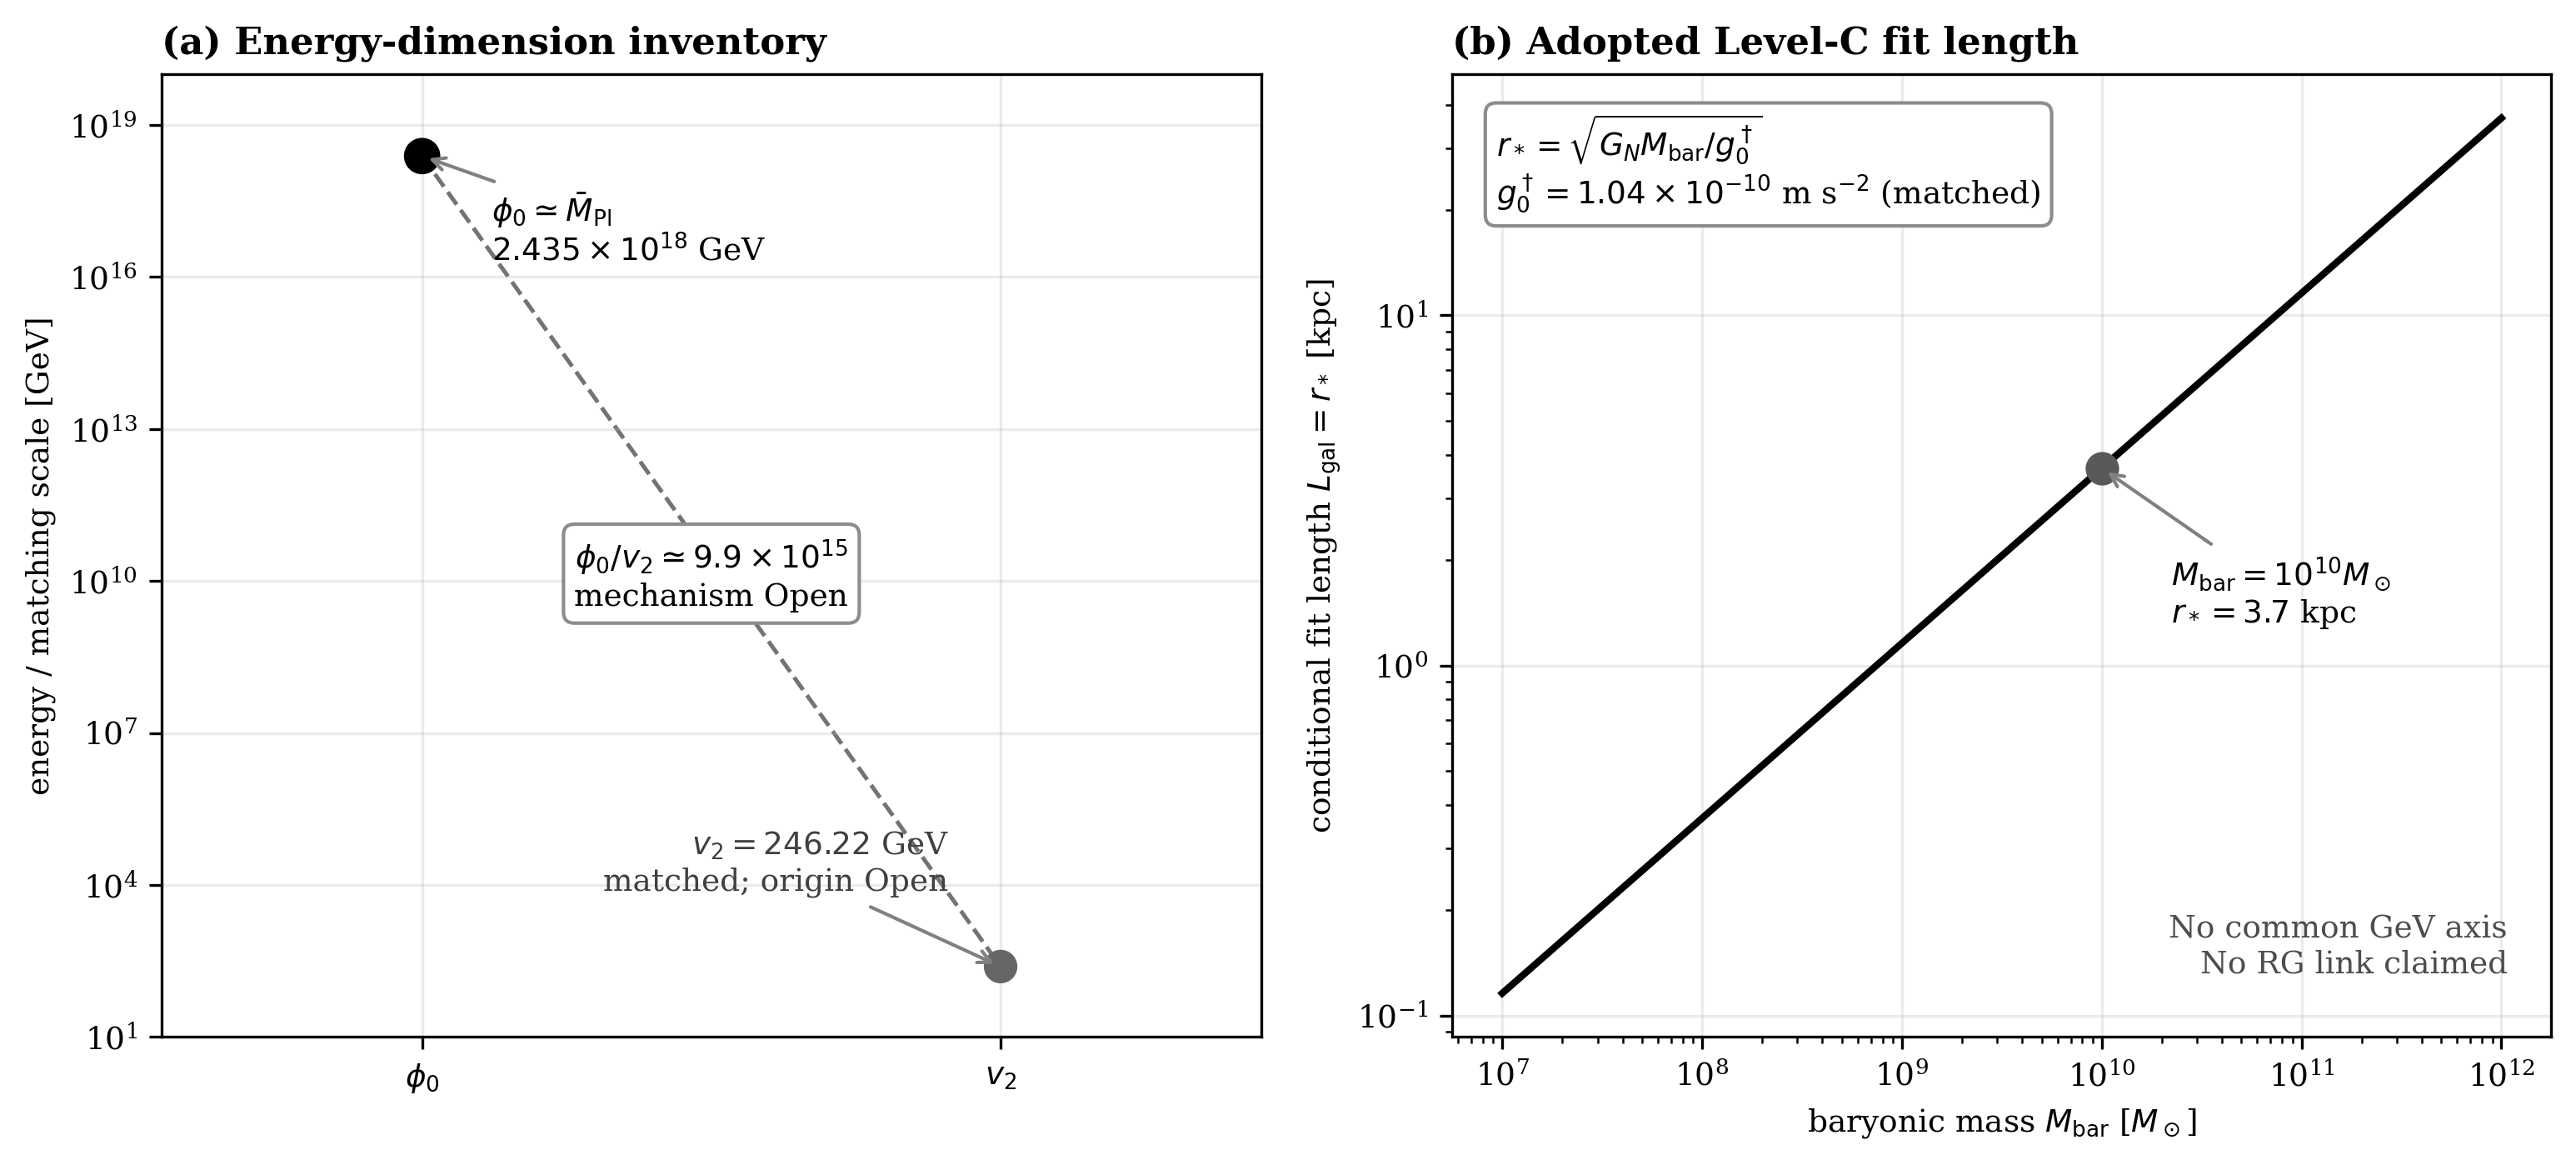
\includegraphics[width=0.92\textwidth]{fig_condensate_scales.png}
\caption{Размерностно разделённый инвентарь. Слева сравниваются два энергетических масштаба $\phi_0$ и $v_2$; градиентная амплитуда $u_0$ имеет размерность GeV$^2$ и связана с ними лишь условной оценкой $u_0\sim\phi_0m_\sigma$. Справа показана отдельная длина $L_{\rm gal}=r_*=\sqrt{G_NM_{\rm bar}/g^\dagger}$ внутри принятого Level-C галактического функционала. Общая RG-цепочка между этими объектами не выведена.}
\label{fig:pop_scales}
\end{figure}

В текущем инвентаре имеются два объекта энергетической размерности,
$\phi_0\sim2.4\times10^{18}$\,GeV и $v_2\simeq246$\,GeV.
Градиентная амплитуда $u_0=|\langle\partial_A\Phi\rangle|$ имеет
размерность GeV$^2$, а не GeV; оценка $u_0\sim\phi_0m_\sigma$
является условной размерностной согласованностью.

Согласование записывается как
\begin{equation}
G_N=\frac{c_*^4}{8\pi M_G^2},\qquad
S_0\leftrightarrow\hbar,\qquad
c_*=\sqrt{\frac{\beta}{\alpha-\beta}},
\label{eq:pop_matching}
\end{equation}
где $M_G\sim\phi_0$ и $S_0\leftrightarrow\hbar$ остаются
отдельными Level-B шагами. Иерархия
$\ln(\phi_0/v_2)\approx36.8$ организует
Open-программу генерации электрослабого масштаба, но конкретный
механизм из P1--P6 не выведен.

Галактический объект имеет другую размерность:
$L_{\rm gal}=r_*=\sqrt{G_NM_{\rm bar}/g^\dagger}$ — это условная
длина перехода внутри принятого Level-C fit-функционала. При
$M_{\rm bar}=10^{10}M_\odot$ она составляет примерно
$3.4$--$3.7$\,kpc; её ECT/скалярное происхождение и закон среды
остаются Open.

\FloatBarrier

\section{Петли ECT, квантование и~происхождение $\hbar$}
\label{sec:pop_loops}

Компактная фаза даёт Level-A существование целочисленных секторов обмотки. Физическая нормировка действия, интерференция и полный дискретный спектр требуют дополнительных matching-шагов и системно-зависимой динамики.

In the coherent sector, the effective order parameter has the polar form $\Phi_{\rm eff} = \rho\,e^{i\theta}$, where $\theta$ is a compact (periodic) phase variable. The single-valuedness requirement (BR1) means that if we transport $\theta$ around any closed loop $\mathcal{C}$ in the Euclidean manifold, it must return to its original value:
\begin{equation}
  \oint_{\mathcal{C}} \partial_A\theta\,dX^A = 2\pi n,
  \qquad n \in \mathbb{Z}.
  \label{eq:pop_winding}
\end{equation}
This is not a quantum axiom --- it is a \emph{topological necessity} for any smooth, single-valued function with compact range.

Топологическим следствием является целочисленная метка обмотки. Внутри принятого compact-phase замыкания кандидатное действие элементарной петли записывается как
\begin{equation}
  S_{\rm loop,min} = 2\pi S_0,
  \label{eq:pop_Sloop}
\end{equation}
where the scale $S_0$ depends on the condensate parameters. Through the matching relation~\eqref{eq:pop_matching}, $S_0$ is identified with $\hbar$ (\emph{Level~B}).

Компактная фаза задаёт целочисленные секторы. Выделенная нормировка $S_0$ относится к эффективному замыканию, а $S_0\leftrightarrow\hbar$ является отдельным Level-B эмпирическим matching-шагом, не топологическим тождеством.

The loop sectors partition the coherent branch into topologically distinct classes indexed by the integer $n$. Configurations in different sectors cannot be continuously deformed into each other. После независимого задания квантовой меры разные секторы могут получать относительные фазы и интерферировать. Одна топология обмотки не выводит меру, произвольные лабораторные паттерны или все квантовые метки (B/Open).


\section{Стрела времени, второй закон и~почему время течёт}
\label{sec:pop_arrow}

In the Euclidean picture, the coordinate $w$ is just one of four equivalent spatial directions. There is no ``forward'' or ``backward'' in $w$, just as there is no ``forward'' in $x$. The arrow of time is not fundamental: it is \emph{emergent}.

ECT constructs the thermodynamic arrow in two stages:

\textbf{Stage 1: directional backbone (\emph{Level~A}).} In the Lorentzian branch, the effective dynamics admits a retarded causal structure: perturbations propagate forward along $w$ inside the emergent light cone. The dissipative kernel of the influence-functional formalism is positive-semidefinite ($\Gamma_{\rm irr} \geq 0$), meaning that off-diagonal histories are \emph{suppressed} rather than amplified. This gives the \emph{directionality} of decoherence.

\textbf{Stage 2: entropy growth (\emph{Level~B}).} Under two additional effective-closure assumptions --- an ohmic spectral density and a Markovian regime --- the coarse-grained entropy satisfies:
\begin{equation}
  \frac{dS_{\rm ent}}{dw} = N_{\rm eff}\,\gamma
  \left(\frac{dq}{dw}\right)^2 \geq 0,
  \label{eq:pop_2ndlaw}
\end{equation}
where $N_{\rm eff}$ is the effective number of environmental modes and $\gamma$ is the decoherence rate per mode. The sign is anchored in the Level~A retarded structure; the explicit formula requires Level~B closure.

The result is a three-regime picture:

At the \emph{cosmological} level, the ordered branch defines the cosmic arrow; the second law holds to overwhelming accuracy.

A large positive decoherence exponent suppresses interference between
specified alternatives, but does not define a universal forward/reverse
trajectory-probability ratio.  Such a ratio requires a named protocol, initial
ensembles, reverse dynamics, and a time-reversal convention.  No universal
$P_{\rm back}/P_{\rm fwd}=e^{-\Gamma}$ law is claimed.

The second law is therefore not an independent postulate in ECT. Its directional backbone is Level~A; its full monotonicity is Level~B. What ECT adds beyond Boltzmann is a \emph{structural explanation} of why the initial condition is special: it is tied to ordered-branch selection (P4), not imposed ad hoc.


\section{Спектр, ветвление, калибровочные симметрии и~частицы}
\label{sec:pop_spectrum_etc}

Protocol-free gamma-crossover figure помещена в карантин: показатели декогеренции зависят от канала, состояния и протокола; универсальный forward/reverse закон и единая ось размещения объектов не выведены.

The ordered condensate supports three classes of excitations, each playing a distinct physical role:

\textbf{Amplitude mode ($\sigma$):} fluctuations of the gradient magnitude $u$ around $u_0$.  The current closure treats this sector as heavy and short-ranged at the matched ordered point; its exact $u$-dependence belongs to the OP-grad/F7 completion.

\textbf{Ориентационный сектор ($\delta n^A$):} наивный Goldstone-счёт сокращается интегрируемостью скалярного базиса. Spin-2 маршрут имеет Level~B/Open, а ковариантное ориентационное действие и физический stress tensor остаются Open. Условный отрицательный результат для тяжёлого исторического радиального прокси не выбирает галактическую ветвь.

\textbf{Phase mode ($\theta$):} In the coherent sector, phase fluctuations connect to gauge fields: the photon emerges as the gauge boson of the $U(1)$ phase symmetry (\emph{Level~A/B after P5}).

The ordered condensate is organised into geometric and coherent descriptions.  Their sector distinction is structural; assigning a sharp quantum--classical boundary at $\Gamma_{\rm loop}\sim1$ is a Level~B reduced-state closure estimate, not a Level-A theorem.

\subsection{Калибровочные симметрии и~четыре фундаментальных взаимодействия}
\label{sec:pop_gauge}

P5 supplies a compact-phase redundancy that supports an Abelian gauge route after the required connection and matter matching. It does not by itself derive every non-Abelian gauge sector.

\textbf{Электромагнитный маршрут (\emph{Level~A/B after P5}):} компактная фаза поддерживает Abelian $U(1)$ connection. Полное локальное Maxwell/matter matching и физическая нормировка относятся к Level~B.

\textbf{Слабый маршрут (\emph{Level~B/Open}):} остаточная ориентационная структура и Hopf-locking дают кандидатную $SU(2)$ архитектуру, но локальное действие, представления материи и электрослабое matching остаются незамкнутыми.

\textbf{Цветовой сектор (\emph{Level~B/Open}):} минимальный $O(4)/O(3)$ сектор не может породить $\mathfrak{su}(3)$ по алгебраической размерности. Цвет требует отдельного P7/внутреннего rank-3 модуля; его физическое действие и matter matching остаются Open.

\textbf{Гравитационный маршрут (\emph{Level~B/Open}):} ориентационная жёсткость является кандидатным оператором; $S_n$, его метрическая вариация и физический $T^{(n)}_{\mu\nu}$ остаются Open.

The ordered-branch EFT also admits a candidate Planck-suppressed fermion--director operator (Level~B classification).  Its coefficient is not derived, a constant single-species vector term may be partly removable, and the quoted spin-precession and $\eta\sim10^{-15}$ values are C/Open target sensitivities rather than predictions.

\subsection{Элементарные частицы}

Спектр следует читать как статусный инвентарь, а не как выведенную перепись частиц природы. Spin-2, Abelian, electroweak, colour, fermion и topological маршруты имеют разные уровни A/B/C/Open; полный локальный SM, массы, поколения, устойчивость и реликтовые количества не выведены. Фундаментальное particle content ECT, включая возможный скрытый сектор, остаётся Open.

Figure~\ref{fig:pop_partI_logic} summarises the derivation logic of Part~I.


\section{Заключение Части~I}

\subsection{Основные результаты}

From six postulates (P1--P6) and one derived branch rule (BR1), the following structures are obtained:

\begin{enumerate}
\item Lorentzian signature $(-,+,+,+)$ from $O(4)\to O(3)$ SSB (\emph{A}).
\item Native sectors retained in the low-energy closure share $c_*$; $c_*=c$ is Level-B empirical matching and extra sectors require separate kinetic checks (\emph{A/B/Open}).
\item Equation hierarchy: Euclidean $\to$ KG $\to$ Schr\"odinger (\emph{A/B}).
\item Retarded arrow-of-time backbone from the ordered branch (\emph{A}); monotonic decoherence/entropy growth requires the influence-functional closure (\emph{B}).
\item Explicit $dS_{\rm ent}/dw\ge0$ inside the influence-functional/environmental closure (\emph{B}); only the retarded backbone is structural.
\item Branching into geometric and coherent sectors (\emph{A}).
\item Compact-phase Abelian $U(1)$ route (A/B); full Maxwell/matter matching remains Level~B.
\item Candidate weak $SU(2)$ architecture (B/Open); minimal $O(4)/O(3)$ cannot supply colour, which requires a separate P7/internal rank-3 module (B/Open).
\item Spin-2 orientation route (\emph{B/Open}); covariant orientation action and stress Open.
\item $S_0 = \hbar$ from compact-phase winding (\emph{B}).
\item Existence of integer compact-phase winding sectors (\emph{A}); physical action normalisation and spectrum reconstruction are B/Open.
\item Director-operator scaling $\beta_5\sim m_f/\bar M_{\rm Pl}$ (B dimensional estimate); physical observability and magnitude Open.
\end{enumerate}

\subsection{Ключевые уравнения и~принципы Части~I}

Effective kinetic tensor: $K^{AB} = \beta\,\delta^{AB} - \alpha\,n^An^B$ (uniqueness theorem).

Propagation speed: $c_* = \sqrt{\beta/(\alpha-\beta)}$.

Matching inventory: $G_N=c_*^4/(8\pi M_G^2)$, $S_0\leftrightarrow\hbar$, and $M_G\sim\phi_0$ as a separate matching step; no direct amplitude-to-action-scale theorem is used.

Compact-phase winding: $\oint \partial_A\theta\,dX^A=2\pi n$ (Level~A sectors); $S_{\rm loop,min}=2\pi S_0$ inside the closure, with $S_0\leftrightarrow\hbar$ only after Level-B matching.

Cross-sector cone universality inside the retained native low-energy closure: $c_{\rm phase}=c_\gamma=c_{\rm GW}=c_*$; $c_*=c$ is Level-B empirical matching.

Second law: $dS_{\rm ent}/dw = N_{\rm eff}\gamma(dq/dw)^2 \geq 0$ inside the influence-functional/environmental closure (Level~B); only the retarded causal backbone is structural.

\subsection{Предсказания Части~I}

GW170817 consistency: $|c_{\rm GW}/c - 1| < 6\times10^{-15}$ (satisfied).

Director-coupling targets: the quoted $\omega_5$ and $\eta\sim10^{-15}$ values are benchmark sensitivities pending coefficient matching and an observable bridge.

LIV: $\Delta t_{\rm GW} \sim 10^{-64}$\,s (Planck-suppressed, currently unobservable).

Casimir coefficient $3/2$ only as a conditional toy estimate for idealised condensate-reflecting boundaries in a provisional three-coordinate soft EFT; $N_G^{\rm phys}=1$ in the current integrable scalar basis, and ordinary metallic plates do not test it.

\subsection{Граф логики Части~I}

\begin{figure}[H]
\centering
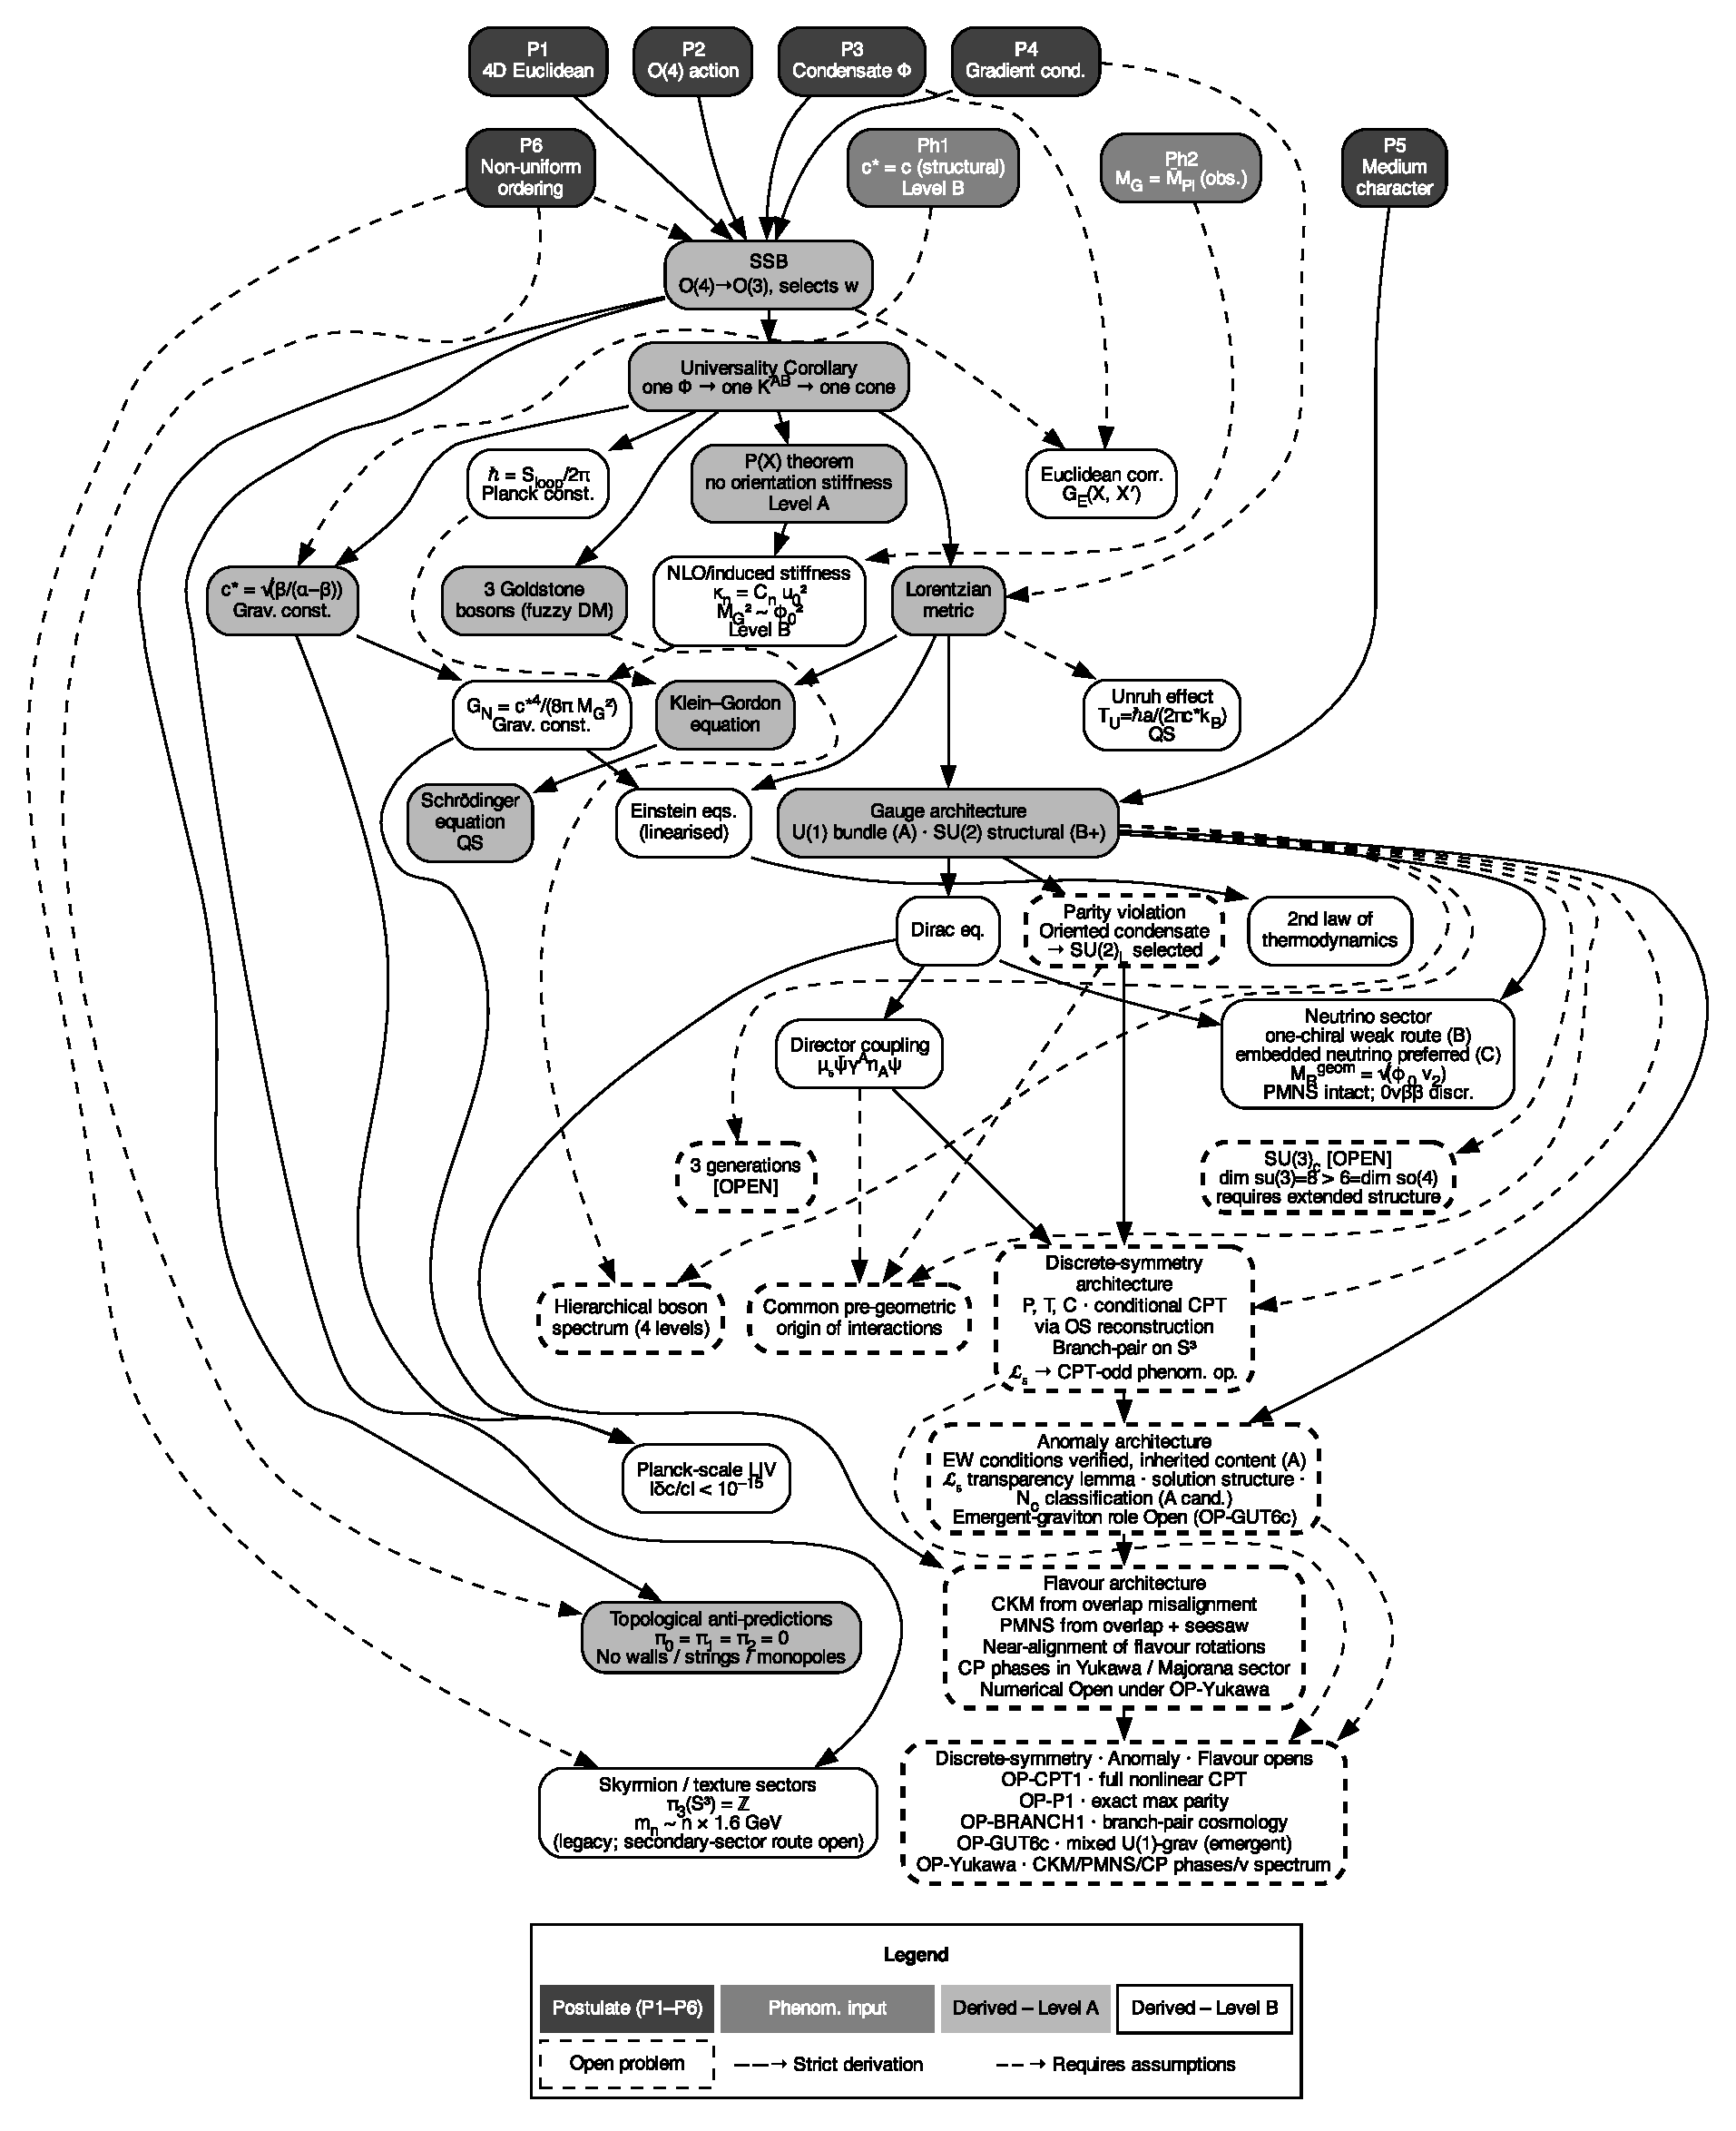
\includegraphics[width=\textwidth]{fig_partI_derivation_logic_pop.pdf}
\caption{Part~I status logic.  The six postulates and BR1 support the Lorentzian-signature result, common-cone and wave-equation routes, the retarded arrow-of-time backbone, the Level-B entropy-growth closure, gauge/particle reconstruction routes, and compact-phase quantisation. Colours distinguish Level~A, B, C, and Open claims.}
\label{fig:pop_partI_logic}
\end{figure}

Figure~\ref{fig:pop_partI_logic} shows the complete derivation architecture of Part~I.

\FloatBarrier

\newpage
%==============================================================
\part{Макроскопическая физика: гравитация, космология и~наблюдательные тесты}
\label{part:macro_pop}
%==============================================================

\section{Специальная теория относительности как однородный предел}

In the homogeneous ordered phase, where the condensate amplitude and direction are uniform throughout space, the effective metric reduces to the Minkowski form: $ds^2 = -c_*^2 dt^2 + dx^2 + dy^2 + dz^2$. All familiar consequences of special relativity follow as theorems: Lorentz transformations arise as the invariance group of the causal cone; time dilation and length contraction are kinematic consequences; $E^2 = p^2c^2 + m^2c^4$ follows from the effective wave equation. In ECT, special relativity is a \emph{derived limit} (\emph{Level~A}), not an independent postulate.


\section{Эмерджентная гравитация и~обобщённые уравнения Эйнштейна}
\label{sec:pop_gravity}

The controlled result relevant here is the scalar-only Jordan-frame ansatz.  In a consistently undivided convention its metric equation has the schematic form
\begin{equation}
  F\,G_{\mu\nu}
  = \frac{8\pi G_N}{c^4}\,T_{\mu\nu}
    + \mathcal{T}^{(q)}_{\mu\nu},
  \label{eq:pop_gee}
\end{equation}
where $\mathcal{T}^{(q)}_{\mu\nu}$ collects the scalar derivative and potential terms.  The factor $G_N/F$ appears only after the entire equation is divided by $F$.

Within the Level~B scalar ansatz, the scalar core uses $a=f_{,q}/f$, $\mathcal A=K+3f_{,q}^2/(2f)$, and $\mathcal E=V_{,q}-2aV-(a/2)\rho_{\rm m}$.  At a stable homogeneous root, $d\ln\bar f/d\rho_{\rm m}=a^2/(2\mathcal E_{,q})\ge0$ and $m_{\rm loc}^2=\mathcal E_{,q}/\mathcal A$ conditionally; this is not finite-body screening.  A frozen homogeneous reference is an algebraic choice, not a screening mechanism or a proof of dynamical reachability.  The displayed action has no independent $n^A$ sector and therefore does not derive $T^{(n)}_{\mu\nu}$.  The candidate $\mathcal X^{\rm cand}_{\mu\nu}[n]$ is only an external proxy.  A physical orientation stress requires a covariant $S_n[g,n,\lambda_n]$, its constraints, and its metric variation (Open); division by $F$ introduces no orientation term.  The quoted FRW, age, Hubble, and JWST diagnostics use the scalar-only background closure.

Следует различать M, S и G: M — микроскопический оператор $\mu_5\bar\Psi\gamma^A n_A\Psi$; S — этот Level-B скалярный анзац; G — независимо принятый Level-C галактический функционал. M$\neq$S по составу переменных, а физический мост S$\to$G (координата, источник, сила, нормировка) остаётся Open. Историческое приложение LOF является смешанным аудитом ветвей: отрицательный результат для тяжёлого радиального прокси не выбирает следующую ветвь, а matter-to-Lorentz-order map остаётся Open.

The galactic, cluster, and cosmological sections below use separate fitted or diagnostic closures.  They do not follow from Eq.~\eqref{eq:pop_gee}.  The body charge, Solar-System profile, PPN projection, exact TT projection, and ghost check are Open.


\section{Эволюция конденсата и~космическая история}
\label{sec:pop_evolution}

\begin{figure}[H]
\centering
\fbox{\parbox{0.86\textwidth}{\centering Superseded visual quarantined after the Round~58 semantic audit; the surrounding status-qualified text is controlling.}}
\caption{Устаревший timeline asset помещён в карантин. Структурно только отсутствие лоренцевых часов до ordering; ordering trajectory, $u_0$ evolution, thermal transfer, inflation replacement и детальная космологическая история остаются B/Open.}
\label{fig:pop_timeline}
\end{figure}

In $\Lambda$CDM, the universe begins at $t=0$ (the Big Bang singularity) and proceeds through inflation, nucleosynthesis, recombination, structure formation, and dark-energy domination. ECT tells a fundamentally different story (Fig.~\ref{fig:pop_timeline}).

Before ordering, the model uses a Euclidean arena without Lorentzian time.  The dimension-two gradient amplitude $u_0$ and the energy-dimension matching scale $\phi_0$ are distinct; no equation sets $u_0=\phi_0$.  The ordering trajectory, branch selection, and any rapid-expansion phase require a nonequilibrium completion and remain Open; inflation is not yet replaced by a derived ECT dynamics.

After the ordering is established, the evolution shares familiar milestones (nucleosynthesis, recombination, galaxy formation), but two features distinguish ECT from $\Lambda$CDM: the gravitational coupling $G_{\rm eff}$ evolves slowly with redshift, and the dark-energy component arises from residual condensate energy rather than from a cosmological constant.

The age integral is a viability discriminator for the retained uniform-$\varepsilon$ diagnostic, not an extraction probe. Two background mappings must remain distinct: approximately $13.5$\,Gyr with the baseline-$H_0$ convention and approximately $12.5$\,Gyr when the shifted inferred $H_0$ is inserted. The mapping choice and full cosmological likelihood remain closure-level/Open.

At late times, ECT admits two scenarios: Scenario~A ($u_0 \to \text{const}$, eternal expansion) and Scenario~B ($u_0 \to 0$, recollapse on a timescale $\sim 10^{100}$\,years). Distinguishing these requires data not yet available.


\section{Четыре классические космологические проблемы}
\label{sec:pop_cosmo_problems}

The standard Big Bang model faces four well-known puzzles. The conventional resolution invokes cosmic inflation --- a brief period of exponential expansion driven by a hypothetical inflaton field. While inflation is remarkably effective, it introduces its own unresolved issues: the inflaton has never been directly observed; inflation requires specific initial conditions to start (the initial homogeneity problem --- inflation itself needs a sufficiently uniform region to begin, yet it was introduced to \emph{explain} homogeneity); the measure problem makes probabilistic predictions ill-defined in the context of eternal inflation; and the trans-Planckian problem arises because CMB modes observed today had sub-Planckian wavelengths at the onset of inflation, potentially probing unknown physics.

ECT supplies distinct structural or conditional non-inflationary routes for these four puzzles.  Their transfer from the pre-ordered Euclidean arena to the observed CMB, including branch selection and the quantitative perturbation spectrum, is not a completed solution and remains Level~B/Open.

\subsection{Проблема горизонта}

The cosmic microwave background (CMB) --- relic radiation from 380\,000 years after the Big Bang --- is uniform to one part in $10^5$ across the entire sky. In $\Lambda$CDM, opposite sides of the sky were never in causal contact at that epoch: their past light cones do not overlap. The uniformity is unexplained without inflation.

Before the $O(4) \to O(3)$ transition the Euclidean arena has no Lorentzian light-cone horizon, giving a structural reframing of the horizon problem (Level~A for that kinematic fact).  Showing that the observed CMB uniformity is dynamically inherited by the selected Lorentzian branch requires an ordering/thermal history and remains Level~B/Open.

\subsection{Проблема плоскости}

Observations show $|\Omega_k| < 0.002$ (Planck 2018). In $\Lambda$CDM, this requires fine-tuning to $\sim 10^{-60}$.

P1 chooses a flat Euclidean substrate ($\delta_{AB}$).  This supplies a candidate non-inflationary flatness route, but it does not by itself prove the curvature of the emergent cosmological branch; the required geometric and dynamical bridge is Level~B/Open.

\subsection{Проблема реликтов и~монополей}

For the minimal vacuum manifold $S^3$, $\pi_2(S^3)=0$ excludes primary stable point monopoles in that sector (Level~A topology). This does not exclude defects from later gauge completions or replace a quantitative relic-production calculation (Open).

\subsection{Проблема первичных возмущений}

The ordered branch carries one independent leading scalar mode (Level~A), but an ordinary $O(4)$-critical correlator projects to a blue tilt.  A conditional Euclidean Lifshitz window can give a flat local seed spectrum $n_\chi=1$; existence of that window and the transfer to the observed $n_s$, $A_s$, and $r$ remain Level~B/Open. The obsolete $n_s\sim0.967$ from an inflationary 60-e-fold proxy is not an ECT prediction.

\subsection{Итог}

The pre-Lorentzian phase provides four non-inflationary structural or conditional routes: no Lorentzian horizon before ordering, a flat substrate, $\pi_2(S^3)=0$ in the minimal sector, and one leading scalar perturbation mode.  Branch selection, emergent curvature, thermal history, and the full $A_s,n_s,r$ prediction remain Open; the present analysis therefore does not establish that inflation is phenomenologically unnecessary.


\section{Тёмный сектор в~ECT}
\label{sec:pop_dark}

The terms ``dark matter'' and ``dark energy'' were introduced phenomenologically to account for observations that standard gravity with visible matter alone cannot explain: flat rotation curves, gravitational lensing, large-scale structure, accelerated expansion. These phenomena are real and well-established. However, the entities postulated to explain them --- invisible particles (WIMPs, axions, sterile neutrinos) and a cosmological constant $\Lambda$ --- have never been directly confirmed despite decades of dedicated searches. The present ECT applications instead use separate fitted or diagnostic closures.  The galactic fit contains no particle-halo term, but this neither derives the full dark sector from the scalar action nor excludes hidden-sector particles.

\subsection{Галактический fit без halo-члена и Open particle content}

In $\Lambda$CDM, the flat rotation curves of galaxies, gravitational lensing in clusters, and the large-scale structure of the universe are attributed to an invisible component --- dark matter particles --- constituting $\sim 27\%$ of the energy budget. Despite extensive experimental programmes spanning direct detection (LUX, XENON, PandaX, LZ), indirect detection (Fermi-LAT, AMS-02), and collider searches (LHC), no dark matter particle has ever been observed. Large regions of the simplest WIMP parameter space are constrained, but no null-search result determines the fundamental ECT particle content or confirms the no-halo fit.

Галактические результаты происходят из практического функционала G (Level~C), а не из исправленного скалярного trace-уравнения или выведенного ориентационного stress tensor.  Rotation curves и BTFR/RAR сохраняют fit/conditional статус.  Отдельный кластерный скрипт является лишь точным аудитом сохранения порядка и argmax для вручную заданных карт и не даёт морфологического свидетельства.  Физический мост S$\to$G и $T^{(n)}_{\mu\nu}$ остаются Open.

\subsection{Тёмная энергия: остаточная энергия конденсата, не~космологическая постоянная}

In $\Lambda$CDM, the accelerated expansion of the universe is attributed to a cosmological constant $\Lambda$ --- a fixed parameter responsible for $\sim 68\%$ of the total energy budget. No fundamental theory explains its value, which differs from quantum field theory estimates by approximately 120 orders of magnitude (the cosmological constant problem).

The value $w_0\approx-0.83$ is a calibrated thawing benchmark anchored to the declared late-time closure, not a parameter-free ECT prediction or a DESI confirmation. A precise result $w=-1$ would reject this present calibrated thawing closure, not the whole ECT framework; a dynamical result would motivate, but not derive, its microscopic origin.

\subsection{Реинтерпретация тёмного сектора в~ECT}

Within the minimal benchmark, the specified galactic interpolation contains no particle-halo term for its fitted mass-discrepancy channel, while the late-time closure uses no rigid external cosmological constant.  This is fit/closure scope only: it neither excludes hidden-sector particles nor establishes that all dark-sector observations follow from the corrected scalar action.


\section{Напряжение Хаббла}
\label{sec:pop_hubble}

\begin{figure}[H]
\centering
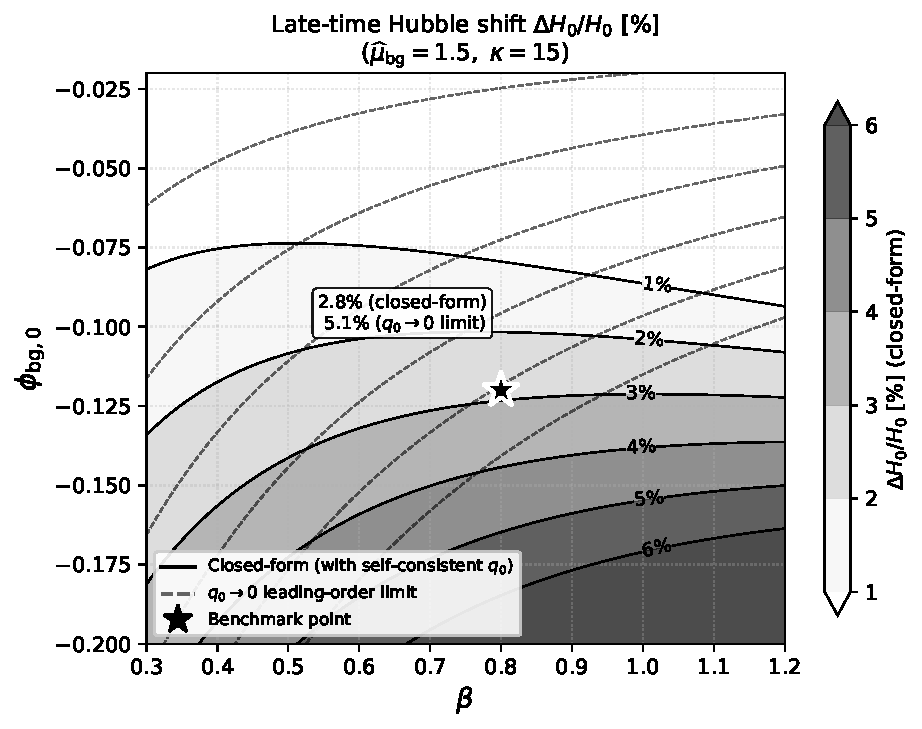
\includegraphics[width=0.82\textwidth]{ect_h0_scan_bw.pdf}
\caption{Uniform-$\varepsilon$ Hubble diagnostic. The retained five-probe band gives an upward baseline-background mapping whose central value is of order the full Planck--SH0ES gap ($\sim5$\,km/s/Mpc). This is a shared diagnostic-layer consistency indicator, not a completed early+late CMB-pipeline resolution; deriving $\varepsilon(z)$ remains Open.}
\label{fig:pop_hubble}
\end{figure}

The Hubble constant $H_0$ measures the current expansion rate of the universe. Two independent methods give discrepant results: the Planck satellite, analysing the CMB assuming $\Lambda$CDM, infers $H_0 = 67.4 \pm 0.5$\,km/s/Mpc; the SH0ES team, using the cosmic distance ladder (Cepheids + Type~Ia supernovae), measures $H_0 = 73.0 \pm 1.0$\,km/s/Mpc. The discrepancy exceeds $5\sigma$ and is known as the \emph{Hubble tension} --- one of the most pressing open problems in cosmology.

The scalar-only diagnostic layer offers an alleviation route (Fig.~\ref{fig:pop_hubble}).  Its fitted high-redshift branch has $G_{\rm eff}(z)>G_N$; this parametrisation is not a finite-body screening result. Specifically, $G_{\rm eff}(z) \approx G_N(1+z)^{2\varepsilon}$, where $\varepsilon$ parametrises the late-time effective drift of the gravitational coupling within the uniform-$\varepsilon$ diagnostic layer. A five-probe cross-consistency analysis in the technical preprint (Hubble + $r_s$, JWST, cosmic chronometers, $f\sigma_8$ from RSD, and ISW), performed under a common background module and the physical prior $\varepsilon \geq 0$, yields a retained joint effective band $\varepsilon \in [0.0296,\,0.0376]$ at $1\sigma$ (centre $\approx 0.033$). At the band central value the upward shift of the CMB-inferred $H_0$ relative to Planck reaches the Planck-SH0ES gap of $\sim 5$\,km/s/Mpc at the baseline-background mapping level, with an accompanying age-viability note. The retained band is an empirical cross-probe consistency window, not a first-principles closure-level prediction; the closure-level derivation of $\varepsilon(z)$ (OP-Hubble-derive in the technical preprint) remains open.

The \emph{sign} of the shift is a structural prediction (\emph{Level~A}): any ordered-branch background with $G_{\rm eff} > G_N$ at high~$z$ necessarily shifts $H_0$ upward. The magnitude is closure-dependent (\emph{Level~B}). The same condensate background simultaneously affects the age budget and early structure formation, producing correlated predictions rather than independent parameters.


\section{Проблема ранних галактик JWST}
\label{sec:pop_jwst}

The James Webb Space Telescope (JWST), launched in December 2021, has detected galaxies at redshifts $z > 10$, when the universe was less than 500 million years old. Several are unexpectedly massive and mature --- containing old stellar populations, organised disk structures, and chemical enrichment that seem to require more formation time than $\Lambda$CDM allows. Standard structure formation with fixed $G_N$ cannot produce such objects quickly enough.

ECT addresses this through two complementary mechanisms, both arising from the same ordered-branch condensate dynamics:

First, the evolving $G_{\rm eff}(z) > G_N$ at high~$z$ means gravitational collapse was \emph{more efficient} in the early universe.

Second, the scalar-only diagnostic closure includes an additional effective response term beyond the uniform $G_{\rm eff}$ drift.  It is a specified diagnostic input, not a calculated orientation stress.

It is important to note that the shorter ECT age (Section~\ref{sec:pop_evolution}) means these high-redshift galaxies had \emph{even less} formation time available than in $\Lambda$CDM --- making the problem nominally worse. Within the scalar-only diagnostic closure, the stronger fitted response and the additional effective term more than compensate: the accelerated collapse rate outweighs the reduced time budget. These are not independent tuning parameters: the same condensate background that shifts $H_0$ upward also enhances early structure formation.


\section{Кривые вращения галактик}
\label{sec:pop_galaxies}

\begin{figure}[H]
\centering
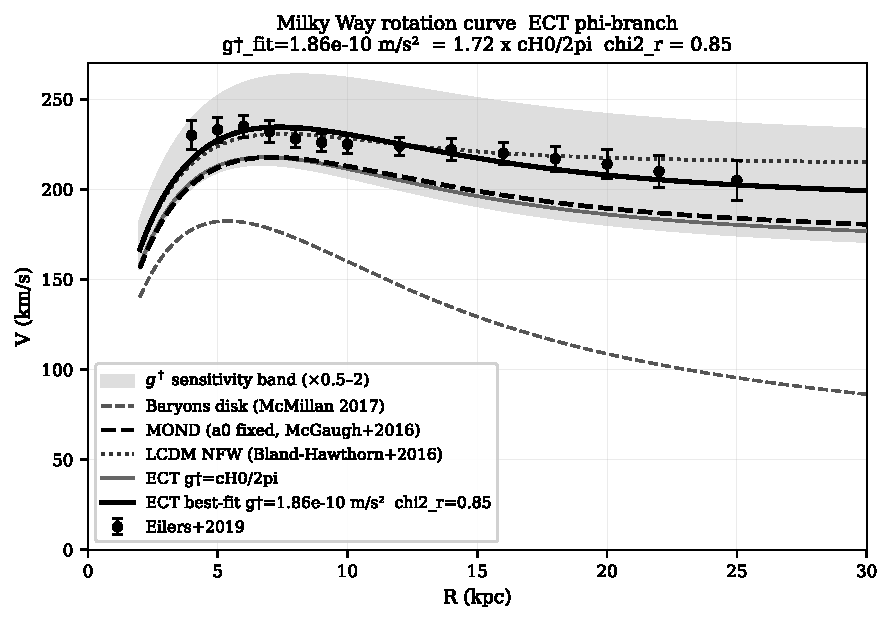
\includegraphics[width=0.82\textwidth]{set1_milky_way.pdf}
\caption{Milky Way rotation curve. The adopted galactic interpolation closure (solid) fits the data with one parameter $g^\dagger_{\rm eff}\approx 1.72\,g^\dagger_0$: $\chi^2/N = 2.95$. Newtonian prediction from baryons alone (dashed) falls off at large radii. (\emph{Phenomenological fit: Level~C.})}
\label{fig:pop_mw}
\end{figure}

When astronomers measure the orbital speeds of stars in spiral galaxies, they find that stars in the outskirts orbit much faster than predicted by the visible matter alone. In a Newtonian calculation, the rotation speed should decrease as $v \propto 1/\sqrt{R}$ beyond the luminous disk, but observations show flat rotation curves extending to many disk radii. The standard explanation invokes a halo of dark matter particles surrounding each galaxy.

Despite decades of direct detection experiments (LUX, XENON, PandaX, LZ, and others), no dark matter particle has ever been observed. Large regions of the simplest WIMP parameter space are constrained, but no null-search result determines the fundamental ECT particle content or confirms the no-halo fit. This persistent non-detection motivates consideration of alternative explanations.

The galactic interpolation is specified and documented as a phenomenological fit closure; it is not derived from the corrected scalar action (\emph{Level~C}).  Its amplitude coordinate $\phi_u=\beta_\phi^{-1}\ln(u/u_\infty)$ is distinct from $\psi_\chi=\ln(\chi/\chi_{\rm vac})$.  The provisional loop result $K_\chi\propto e^{-\psi_\chi/2}$ cannot determine the $\phi_u$ coefficients or derive the AQUAL branch without a $u\leftrightarrow\chi$ map.  Finite-body screening, body charge, and Solar-System reachability remain Open.  The adopted interpolation is:
\begin{equation}
  g(R) = \tfrac{1}{2}\bigl(g_N + \sqrt{g_N^2 + 4\,g_N\,g^\dagger}\bigr),
  \label{eq:pop_interp}
\end{equation}
with the matched reference $g^\dagger_0\sim cH_0/(2\pi)\approx1.04\times10^{-10}$\,m/s$^2$; per-galaxy $g^\dagger_{\rm eff}$ values are Level-C fit outputs.  The deep- and strong-field limits are algebraic properties of this closure, not a derivation of the physical branch or finite-body screening.  Отдельно, показанная кривая force-law dimensionality предполагает иллюстративную point-source альтернативу $\mu_{\rm dim}=x/\sqrt{1+x^2}$, а не практический функционал G. Проверка на протяжённых галактиках требует измеренного локального $p_N(r)$ и пока не выполнена (Level~C algebra / Open test).

\begin{figure}[H]
\centering
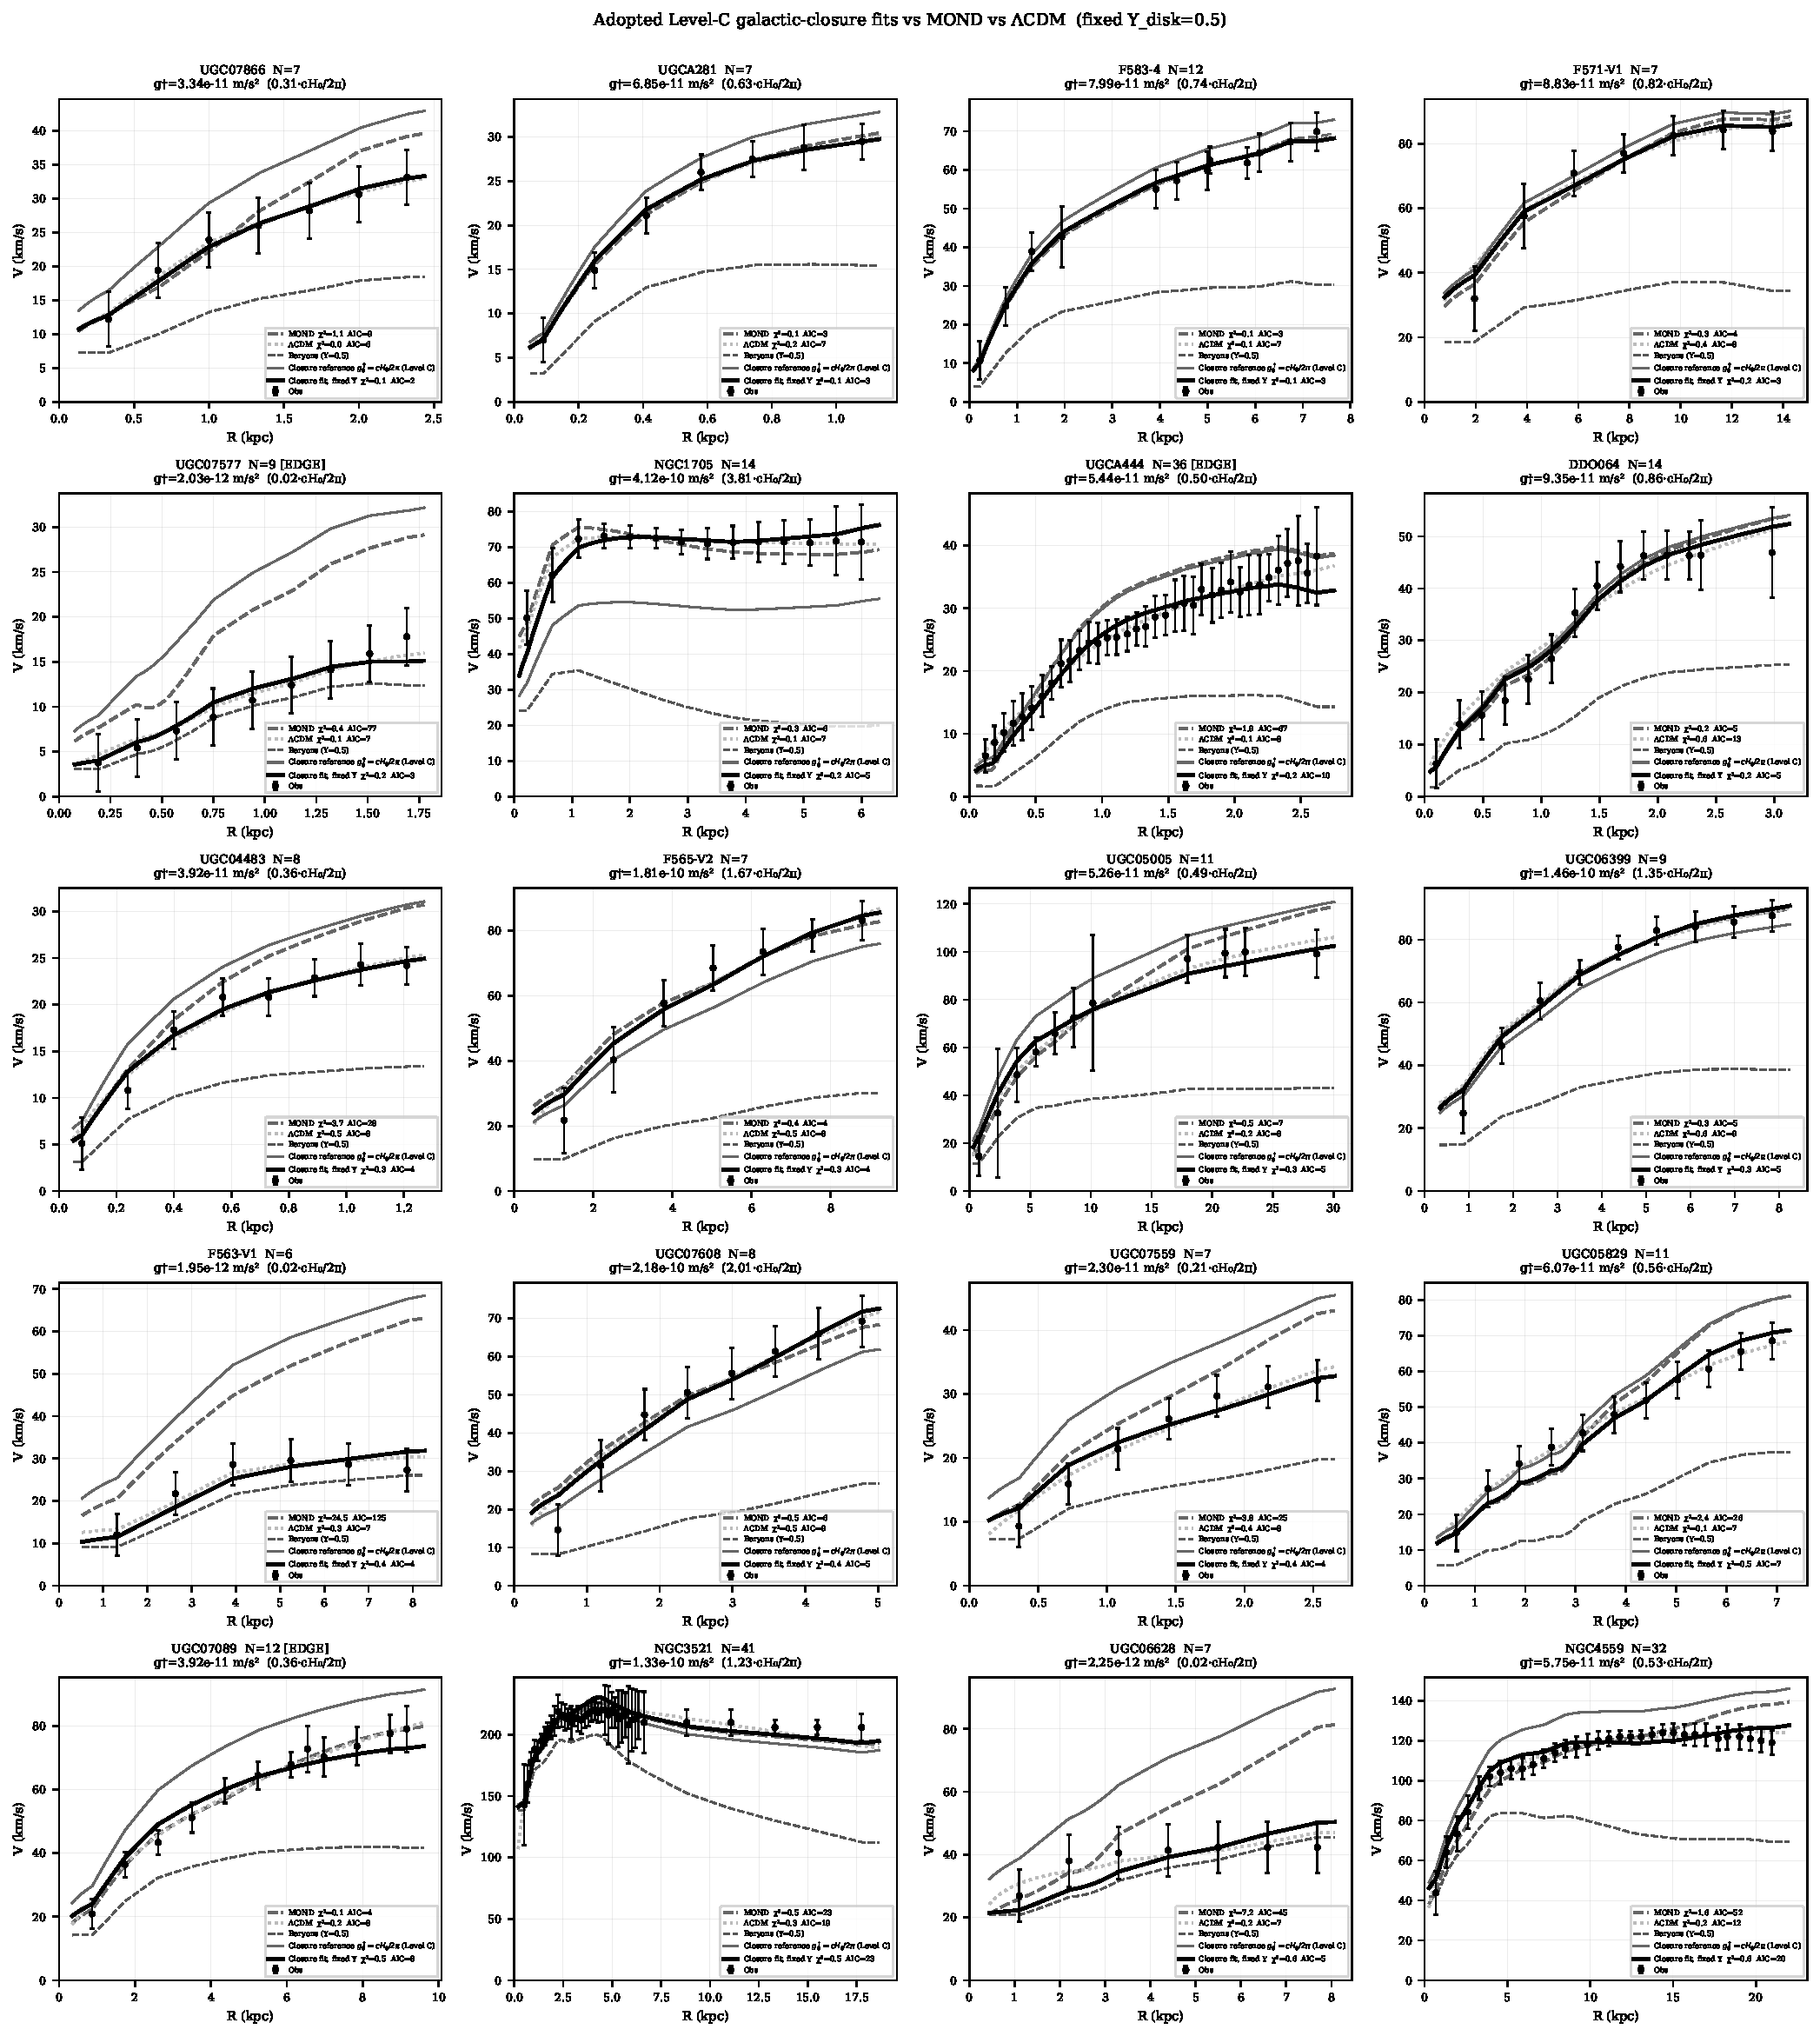
\includegraphics[width=\textwidth]{set2_sparc_sample.pdf}
\caption{Rotation-curve fits for a sample of SPARC galaxies, spanning a wide range of morphologies: from dwarf irregulars to massive spirals. The adopted interpolation closure (solid) uses one fitted parameter per galaxy. (\emph{Level~C.})}
\label{fig:pop_sparc}
\end{figure}

This phenomenological closure has been fitted to \textbf{165 galaxies from the SPARC database} (Fig.~\ref{fig:pop_mw}, \ref{fig:pop_sparc}).  The sample medians are $\chi_r^2\approx2.7$ for fixed $M/L$ and $\approx1.4$ for free $M/L$, versus the quoted MOND comparator $\approx3.1$ on comparable parameter footing.  The values $2.95/6.55$ describe only the displayed Milky-Way benchmark.  These are Level~C fit diagnostics, not a scalar or environment-law derivation.

\FloatBarrier

\section{Барионное соотношение Талли--Фишера и~RAR}

\begin{figure}[H]
\centering
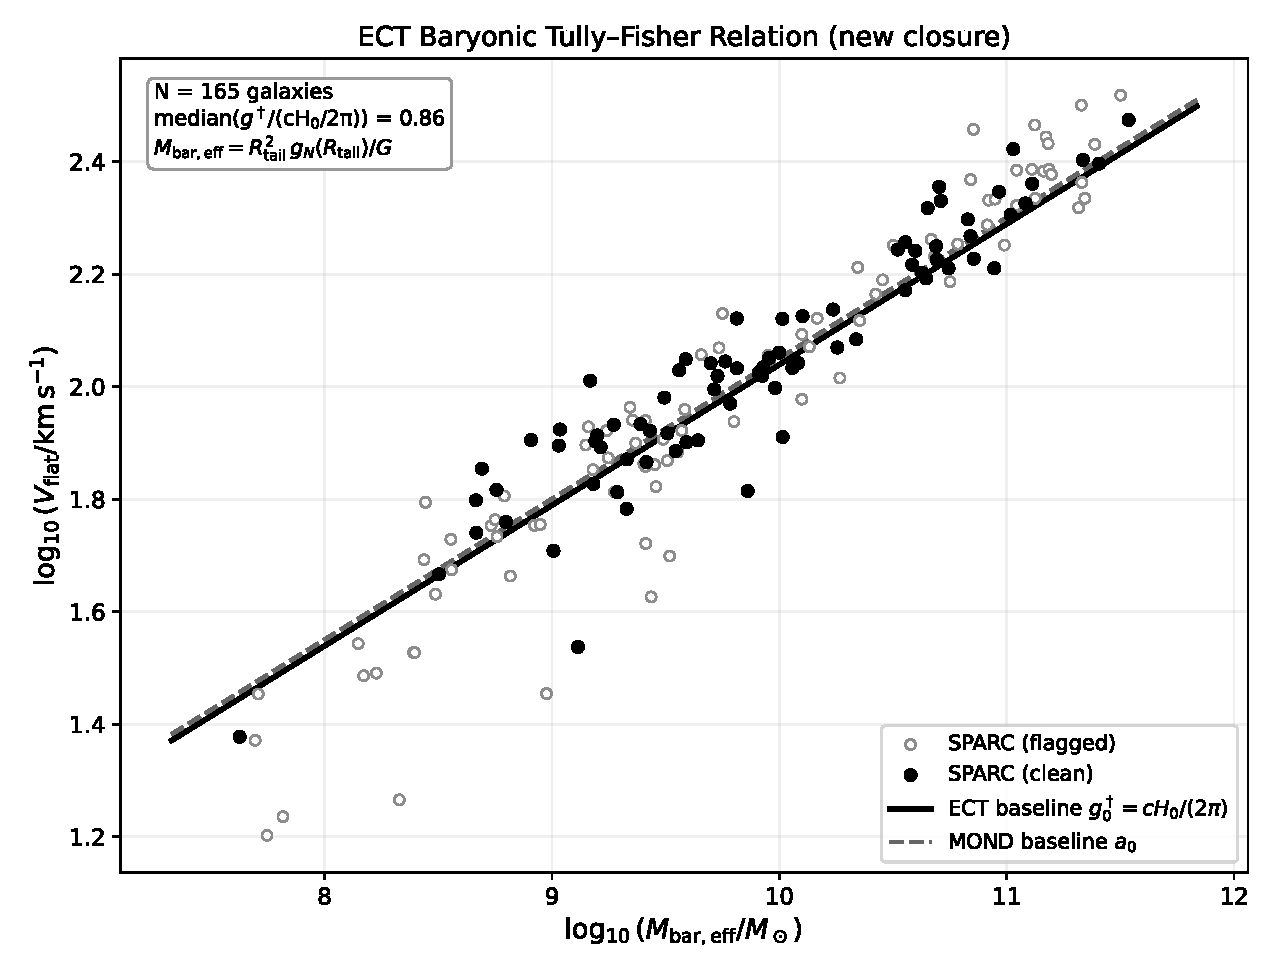
\includegraphics[width=0.88\textwidth]{ect_btfr_new_bw.pdf}
\caption{The baryonic Tully--Fisher relation (BTFR) from the SPARC sample. Within the adopted deep-branch closure, the algebra gives slope~4 (solid line): $v_{\rm flat}^4 = G_N M_{\rm bar}\,g^\dagger$. (\emph{Slope: Level~B/C conditional on the closure; fitted $g^\dagger$ value: Level~C.})}
\label{fig:pop_btfr}
\end{figure}

The BTFR --- $M_{\rm bar} \propto v_{\rm flat}^4$ --- is one of the tightest empirical correlations in extragalactic astronomy (Fig.~\ref{fig:pop_btfr}).  Within the adopted ECT deep-branch closure, $v_{\rm flat}^4 = G_N M_{\rm bar}\,g^\dagger$ and slope~4 follow algebraically.  Selection of that physical branch and its fitted normalization remain Level~B/C, not Level~A.

\begin{figure}[H]
\centering
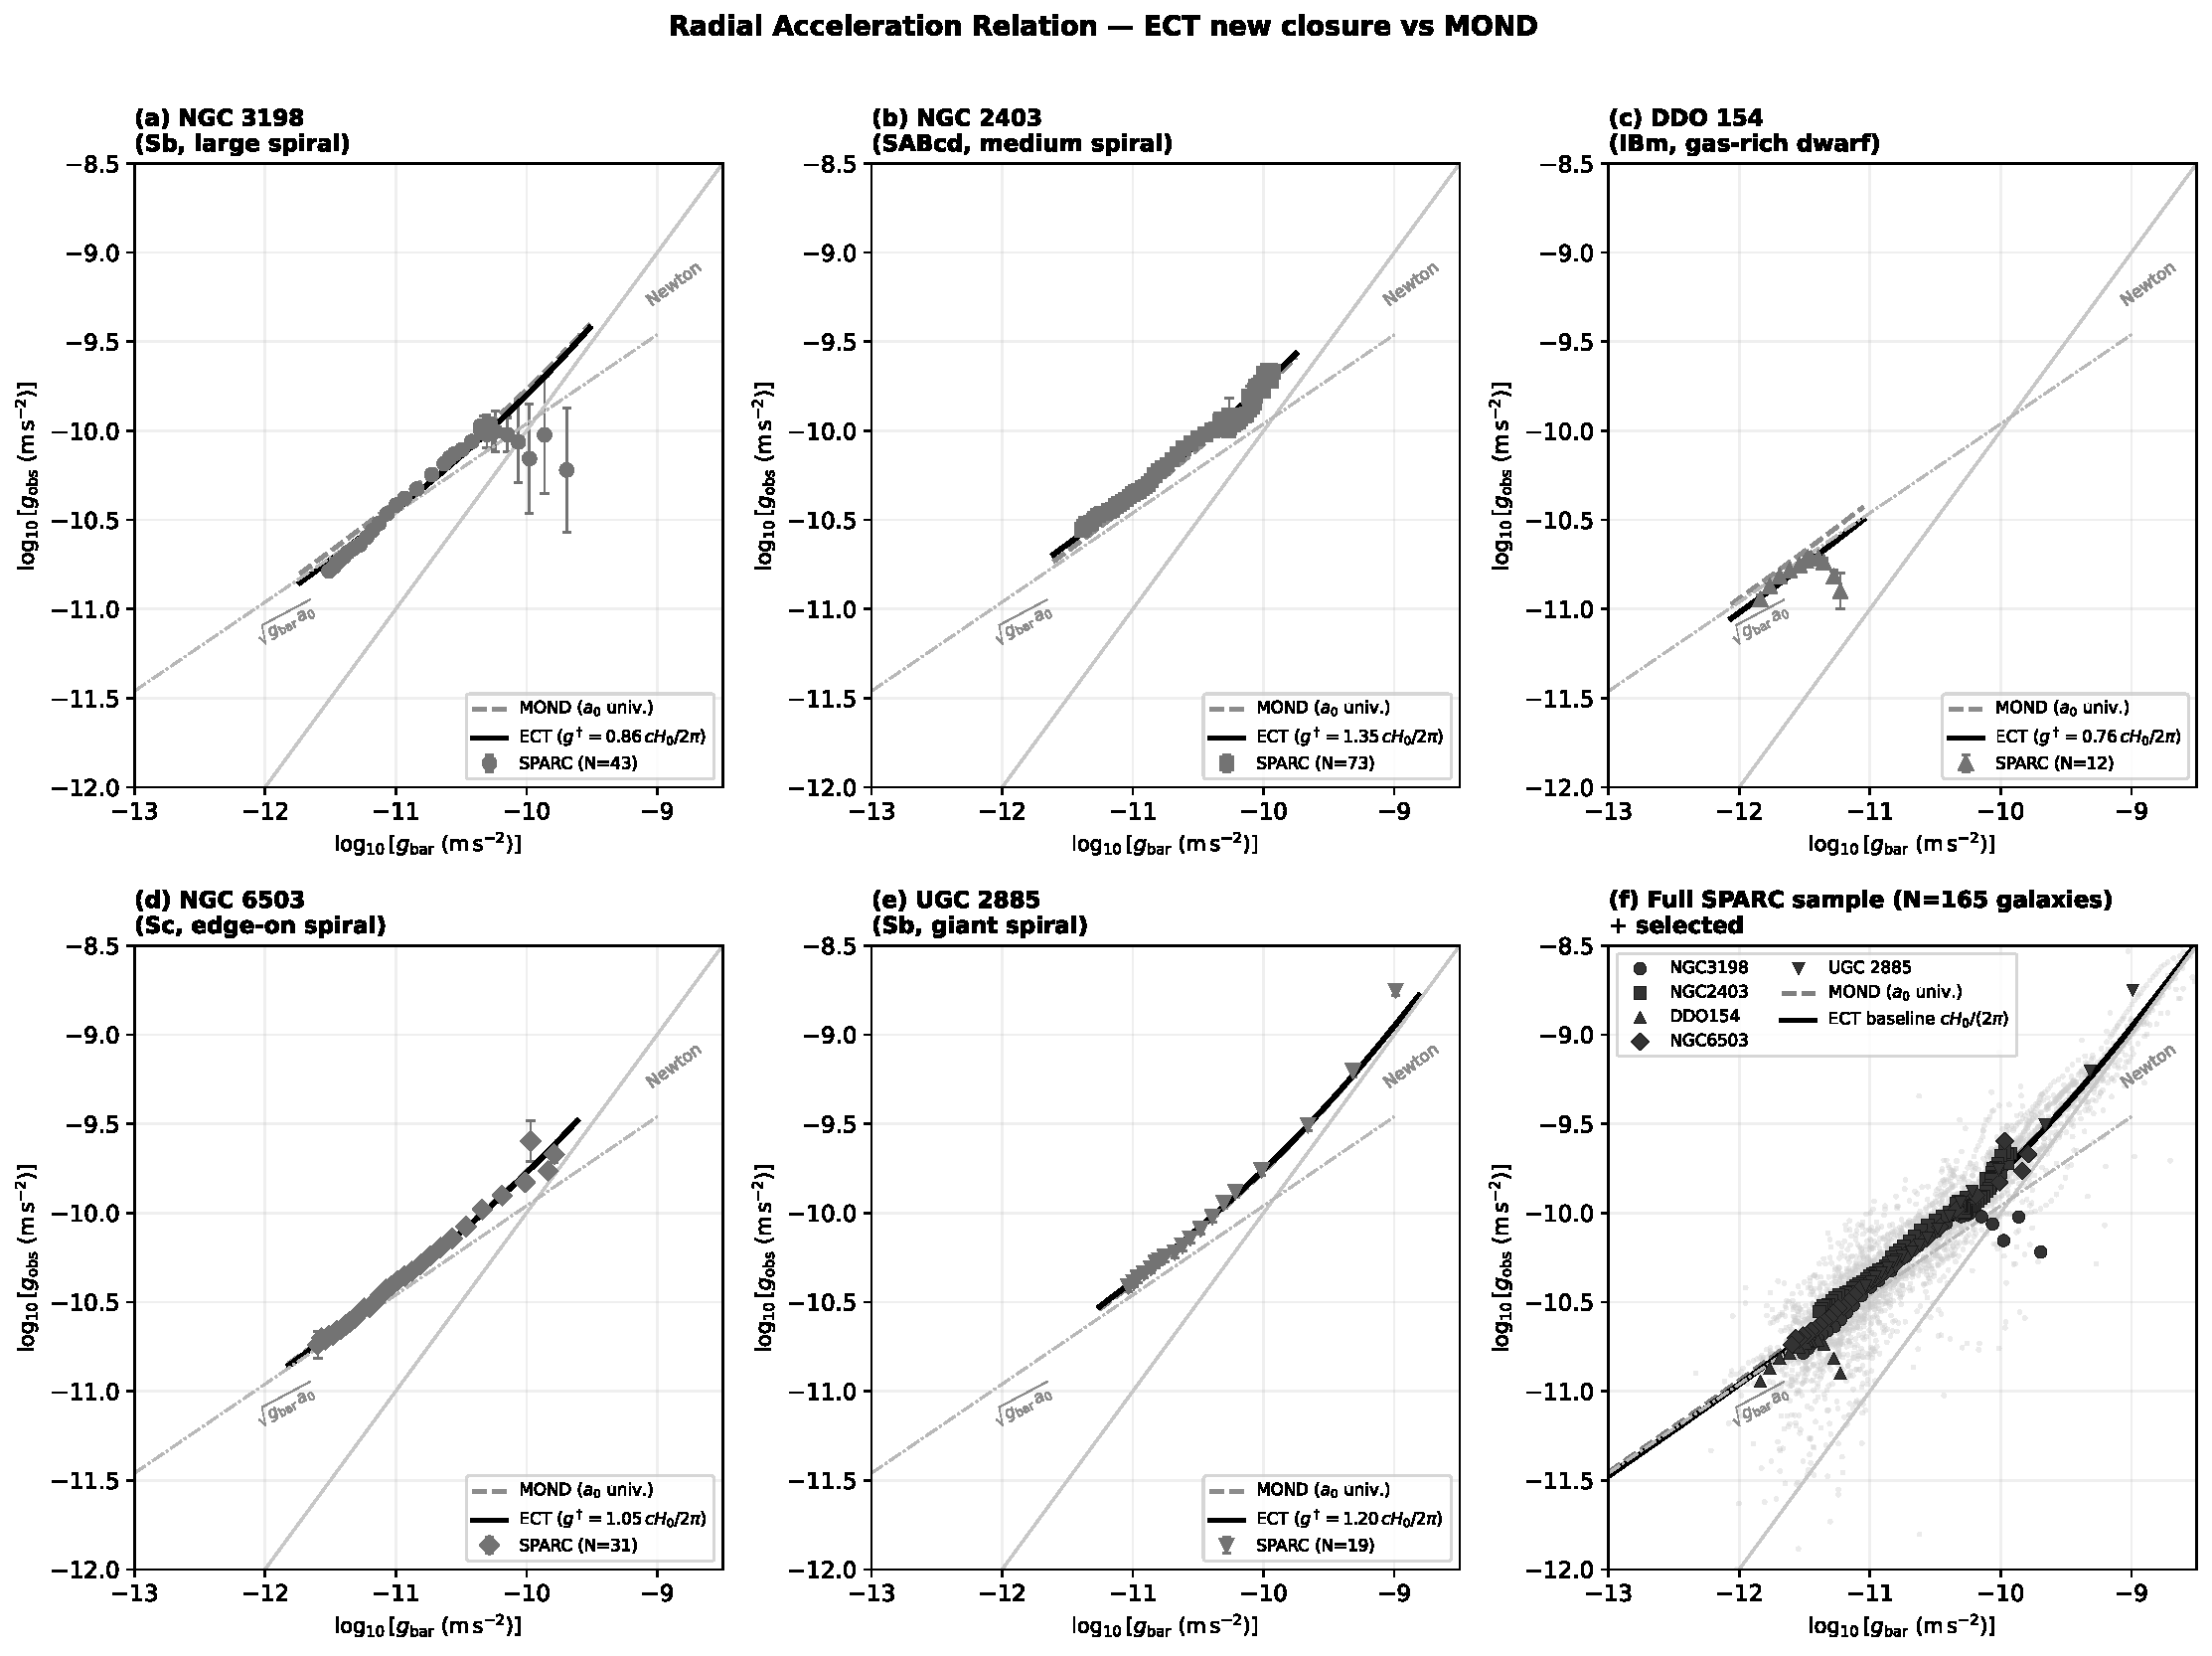
\includegraphics[width=\textwidth]{ect_rar_new_6panel_bw.pdf}
\caption{RAR diagnostics from the SPARC sample.  The adopted closure is compared with the matched reference $g^\dagger_0\approx1.04\times10^{-10}$\,m/s$^2$ and the empirical scale $a_0\approx1.2\times10^{-10}$\,m/s$^2$.  Per-galaxy $g^\dagger_{\rm eff}$ values are Level~C fit outputs; the RAR is not an independent test of the same closure.}
\label{fig:pop_rar}
\end{figure}

The RAR (Fig.~\ref{fig:pop_rar}) is reproduced by the adopted interpolation law~\eqref{eq:pop_interp}; it is not an independent bare-theory prediction.  An environment/history factor $\Xi$ is an exploratory Open hypothesis with no derived sign or amplitude.

\FloatBarrier

\paragraph{UDG inverse diagnostic после аудита нормировки Wolf.}
При $R_{1/2}=4R_e/3$ используется изотропный прокси
$M_{\rm dyn,1/2}=3\sigma_{\rm los}^2R_{1/2}/G$ и
$M_{\rm bar,1/2}=M_\star/2$. Для
$\mathcal R_{\rm dyn}=g_{\rm obs}/g_N$ инверсия практического функционала G
даёт
\[
\Xi_{\rm alg}=\mathcal R_{\rm dyn}(\mathcal R_{\rm dyn}-1)
\frac{g_N}{g^\dagger_0}.
\]
Это неограниченный алгебраический диагностик, а не предсказанный фактор среды;
физическая область требует $\Xi_{\rm alg}\ge0$. Центральные значения равны
$-0.00369$ для DF4 (нет физического неотрицательного решения), $0.00516$ для
FCC~224, $0.892$ для NGC~5846-UDG1 и $4.981$ для Dragonfly~44; dispersion
bracket DF2 даёт $0.031$--$0.423$. Прежняя общая логарифмическая 95\%-полоса
отозвана. Boundary-aware Jeans likelihood и закон среды остаются Open.

\begin{figure}[H]
\centering

\includegraphics[width=0.92\textwidth]{fig_udg_regime_diagram.pdf}
\caption{UDG acceleration-residual proxy с нормировкой Wolf~3. Он проверяет
принятый Level-C функционал, не задаёт микроскопическую скалярную координату и
не является результатом screening.}
\label{fig:pop_udg_regime}
\end{figure}

\begin{figure}[H]
\centering

\includegraphics[width=0.92\textwidth]{fig_udg_stress_test.pdf}
\caption{Исправленный $\Xi_{\rm alg}$ inverse diagnostic. Маркер DF4 означает
отсутствие физического $\Xi\ge0$ при центральных входах; интервалы дисперсии
являются граничными проверками, а не общей 95\%-posterior.}
\label{fig:pop_udg}
\end{figure}

\FloatBarrier

\section{Аудит проекционного кластерного прокси}
\label{sec:pop_clusters}

Текущий скрипт применяет строго локальное отображение
$\Sigma_{\rm cl}=\Sigma_b\nu_{\rm cl}(2\pi G_N\Sigma_b/g^\dagger_{\rm cl})$
к вручную заданным гауссовым барионным картам. Для
$D=\sqrt{1+4/y^2}$ точно выполняется
\[
\frac{d\ln\Sigma_{\rm cl}}{d\ln\Sigma_b}
=\frac{D+1}{2D}\in(1/2,1),
\qquad
\arg\max\Sigma_{\rm cl}=\arg\max\Sigma_b.
\]
Следовательно, преобразование сохраняет порядок всех положительных пикселей
и сжимает контраст. Класс пика BCG/gas уже задан входной картой; четыре
системы являются проверкой реализации, а не воспроизведением морфологии,
линзирования или свидетельством в пользу ECT.

\begin{figure}[H]
\centering

\includegraphics[width=0.82\textwidth]{fig_bullet_main.png}
\caption{Аудит локальной карты Bullet Cluster. Совпадение пиков следует
из точной монотонности; нормировочные и ориентационные величины являются
вручную заданными/внешними прокси, а не наблюдаемыми mass ratios.}
\label{fig:pop_bullet}
\end{figure}

\begin{figure}[H]
\centering

\includegraphics[width=\textwidth]{fig_cluster_suite_budget.png}
\caption{Четырёхсистемный аудит сохранения порядка и argmax с игрушечными
гауссовыми барионными входами. $A_0^{\rm proxy}$ и
$A_{\rm fin}^{\rm proxy}$ — детерминированные чувствительности ручной
нормировки, а не наблюдательные амплитуды.}
\label{fig:pop_clusters}
\end{figure}

Физический тест скоплений требует независимо ограниченных барионных карт,
выведенного из действия source/lensing response (возможно нелокального) и
заранее заданного внешнего likelihood. Всё это остаётся Open.

\section{Асимметрия материи и~антиматерии}

The observable universe contains far more matter than antimatter: $\eta_B^{\rm obs} \approx 6 \times 10^{-10}$. This asymmetry requires baryon number violation, $C$/$CP$ violation, and departure from thermal equilibrium (the three Sakharov conditions, 1967). The Standard Model satisfies these conditions in principle but cannot quantitatively produce the observed asymmetry.

ECT содержит кандидатные ингредиенты, совместимые с тремя условиями Сахарова только внутри заявленных эффективных замыканий (Level~B): ordering transition, кандидатный CP-odd/director сектор и topology-changing каналы. Их одновременная физическая реализация и ECT-native расчёт бариогенеза остаются Open. Значение $\eta_B\sim9\times10^{-10}$ является внешним benchmark, а не предсказанием ECT.





\section{Заключение Части~II}

\subsection{Основные результаты}

From the ordered-branch EFT, the geometric branch produces:

\begin{enumerate}
\item Special Relativity as the homogeneous limit (\emph{A}).
\item Scalar-only metric normalization inside its ansatz; $T^{(n)}_{\mu\nu}$ requires covariant $S_n[g,n,\lambda_n]$ and remains Open.
\item Four non-inflationary structural/conditional routes; quantitative cosmological completion remains Open (\emph{A/B/Open}).
\item Calibrated thawing benchmark $w_0\approx-0.83$ inside the declared late-time closure (C/B-closure); microscopic origin Open.
\item Hubble diagnostic: retained $\varepsilon$ band maps upward by about the full baseline gap near its centre; shared-module indicator only, with full pipeline and $\varepsilon(z)$ derivation Open.
\item JWST diagnostic: enhanced $G_{\rm eff}$ plus an adopted closure term (\emph{B/C}; orientation Open).
\item 165 SPARC galaxies: median $\chi_r^2\approx2.7$ for fixed $M/L$ and $\approx1.4$ for free $M/L$, versus the quoted MOND comparator $\approx3.1$ on comparable footing (\emph{C}).
\item BTFR slope exactly 4 conditional on the adopted deep-branch closure (\emph{B/C}).
\item RAR fit with $g^\dagger \approx cH_0/(2\pi)$ (\emph{C}); physical matching and $\Xi$ are Open.
\item Тождество сохранения порядка/argmax локального кластерного прокси (Level~C algebra); физический тест линзирования и морфологии Open.
\item Baryogenesis: Sakharov-compatible ingredients exist in declared closures (B); an ECT-native $\eta_B$ derivation is Open.
\item Level-C галактический fit без halo-члена и отдельное калиброванное поздневременное скалярное замыкание; их ECT-мост, particle content и общий микроскопический источник Open.
\end{enumerate}

\subsection{Ключевые уравнения и~принципы Части~II}

Scalar-only metric equation (undivided): $F G_{\mu\nu}=8\pi G_N T_{\mu\nu}/c^4+\mathcal T^{(q)}_{\mu\nu}$; division by $F$ adds no orientation term, and $T^{(n)}_{\mu\nu}$ requires covariant $S_n[g,n,\lambda_n]$ (Open).

Galactic interpolation: $g(R) = \frac{1}{2}(g_N + \sqrt{g_N^2 + 4g_Ng^\dagger})$.

BTFR: $v_{\rm flat}^4 = G_N M_{\rm bar} g^\dagger$ (slope 4, algebraic).

$G_{\rm eff}(z) \approx G_N(1+z)^{2\varepsilon}$, retained $\varepsilon \in [0.0296,\,0.0376]$ at $1\sigma$ (Hubble shift).

\subsection{Наблюдательные тесты и~фальсификаторы}

ECT is falsifiable. Key predictions of the macroscopic sector:

\begin{itemize}
\item BTFR slope = 4 conditional on the adopted closure (\emph{B/C}); fitted $g^\dagger \sim cH_0/(2\pi)$ (\emph{C}).
\item Director-operator form is Level~B, while $\eta\sim10^{-15}$ is only a C/Open target sensitivity pending coefficient and observable-bridge matching; dark energy $w_0\approx-0.83$ retains its calibrated closure status.
\item Exploratory environment/history law $\Xi$ (\emph{Open}); $M_{\rm max} = 2.17\,M_\odot$ (\emph{B}).
\item CMB quadrupole deficit (\emph{B/Open}).
\end{itemize}
Full list with explanations is given in Part~IV, Section~\ref{sec:pop_predictions}.

Устаревшее изображение cosmology-predictions помещено в карантин: его встроенные $\varepsilon$, $\Delta H_0$ и $w_0$ метки предшествуют аудиту retained-band/shared-diagnostic статуса.

\subsection{Граф логики Части~II}

\begin{figure}[H]
\centering
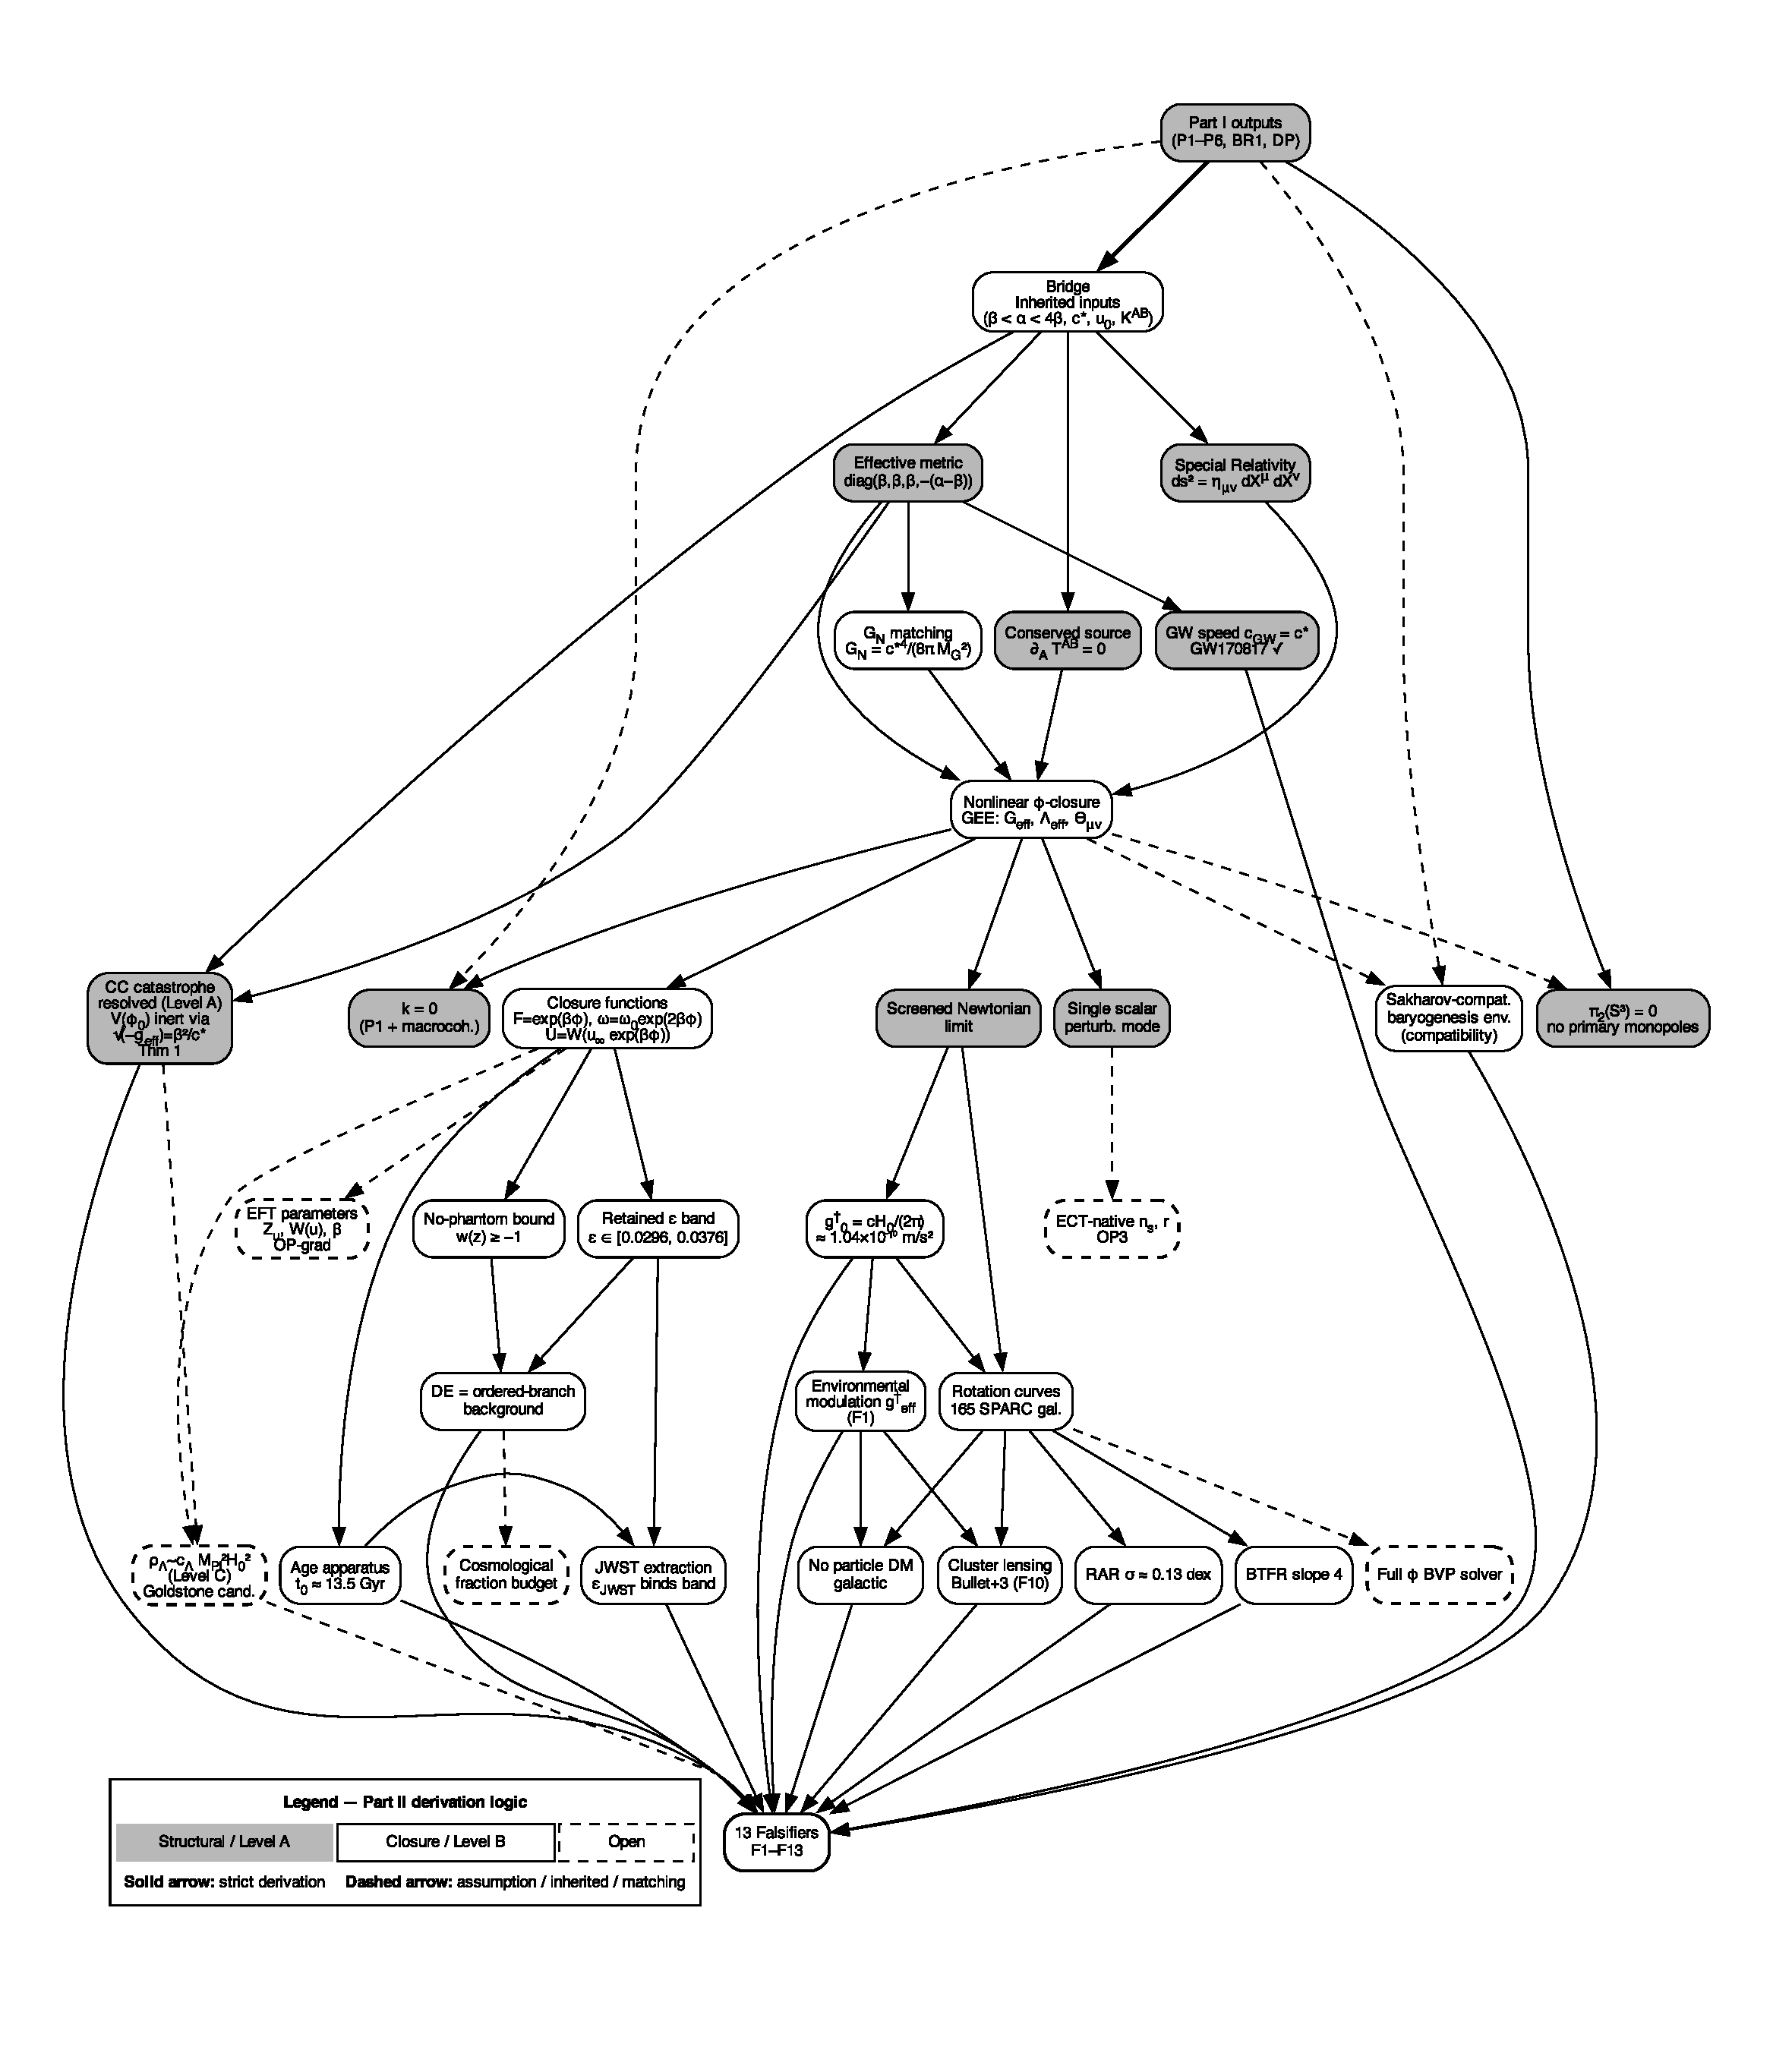
\includegraphics[width=\textwidth]{fig_partII_derivation_logic_pop.pdf}
\caption{Part~II status and dependency map.  It distinguishes strict ordered-branch statements from Level-B/C diagnostic closures and Open physical bridges; it does not imply that all macroscopic entries follow from one action.}
\label{fig:pop_partII_logic}
\end{figure}

Статусно разделённая логика Части~II показана на рис.~\ref{fig:pop_partII_logic}; устаревший cosmology-prediction visual помещён в карантин, поэтому controlling является текст выше.

%==============================================================
\part{Квантовый сектор: когерентная ветвь}
\label{part:quantum_pop}


\section{ECT versus стандартная квантовая механика}
\label{sec:pop_ect_vs_qm}

Устаревшее ECT-versus-QM изображение помещено в карантин: его встроенные Born и measurement метки превышают conditional C1--C3/Open статус.

Standard quantum mechanics supplies a tested operator/probability
framework. ECT offers reconstruction routes from selected Euclidean coherent
subsectors, but the interacting states, Born weights without C1--C3, detector
updates, solution uniqueness, and a measure over solutions remain B/Open. The
boundary-value formulation is therefore an architectural hypothesis, not a
proof that probability is only coarse-graining.

\textbf{The hydrogen atom.} ECT currently offers a Level-B structural interpretation in which regular phase-consistent solutions can support discreteness. It has not derived the Coulomb Hamiltonian, the $-13.6/n^2$\,eV spectrum, fine structure, or $\alpha_{\rm fs}$ from the minimal action; those quantitative steps remain Open.

\textbf{The double-slit experiment.} Admissible Euclidean solutions or an ensemble may depend on declared apparatus boundary data, but ECT has not established uniqueness, a physical measure, the detector map, or the observed $|\psi_1+\psi_2|^2$ probabilities. This is B/Open interpretive compatibility, not an ECT-native fringe calculation.

\textbf{Measurement.} The detector belongs to the full boundary-value problem.  At reduced-description level, environmental coupling can suppress interference and support classical record formation ($\Gamma_{\rm loop}\gg1$; Level~B).  Decoherence alone does not derive a unique pointer basis or select one ontologically actual outcome; those steps and a complete update theorem remain Open.

\textbf{Conditional field-level determinism.} The Euclidean equation defines a classical nonlinear boundary-value problem after a branch and admissible data are specified. Global existence, uniqueness, stability, and a measure/selection rule over multiple solutions are not proved. The no-fundamental-collapse ontology is architectural; subsystem probabilities, Born weights, and measurement remain B/Open.

\textbf{Boundary dependence and delayed-choice compatibility.} Interior solutions of a well-posed elliptic problem can depend on all specified boundary data. Mapping laboratory settings to physical ECT boundary data and reproducing delayed-choice/eraser probabilities and no-signalling remain Open. This is interpretive B/Open compatibility, not a future-setting or retrocausal derivation.

\textbf{Unified origin of coherent and geometric branches.} A central structural claim of ECT: gravity and quantum coherence are not separate ingredients forced together, but two sectors of one ordered condensate. The long-wavelength sector is read geometrically (gravity); the coherent shorter-wavelength sector is read wave-mechanically (quantum). This is not ad hoc stitching --- it follows from the mode decomposition of the same condensate around the same ordered background (\emph{Level~A}).

\begin{sloppypar}
\textbf{What ECT already reproduces or structurally organises:} Coherent-sector results include Schr\"odinger/KG limits, compact phase, environmental decoherence, measurement and spin routes, PES, tunnelling/entanglement bridges, and $S_0$ matching.

The gravitational record channel is Open; its current D--P numbers are external benchmarks.
\end{sloppypar}

\textbf{What remains open:} Born rule from first principles; complete measurement theorem; Bell correlators from condensate theory; three generations; $\alpha_{\rm fs} = 1/137$; full Yukawa hierarchy. These are open derivational targets, not failures of the framework.


\section{Структура гильбертова пространства из рефлексивной положительности}

Where reflection positivity has been verified in the Gaussian/free quadratic coherent subsectors, Osterwalder--Schrader reconstruction yields a Hilbert space with positive inner product and unitary evolution. Extending this result to the full interacting coherent branch and deriving the complete canonical operator algebra remain B/Open.

Standard QM uses the Osterwalder--Schrader theorem in the \emph{opposite} direction: starting from a quantum theory, it checks that the Euclidean continuation is well-defined. ECT uses it \emph{constructively}: starting from the Euclidean condensate, it \emph{builds} the Hilbert space. The quantum formalism is constructed, not assumed.


\section{Суперпозиция, интерференция, обменная статистика и~принцип Паули}

\textbf{Linear superposition route} (\emph{A inside the quadratic subsector; B/Open physically}): linearised solutions can be added, but the full interacting quantum-state principle still requires RP/OS and operator completion.

\textbf{Interference route} (\emph{B/Open}): compact phase and matched path-integral weighting provide a route to interference; topology alone does not derive the full measure or arbitrary laboratory patterns.

\textbf{Exchange statistics} (\emph{Level~A/B}): Connected to the topology of path configurations in the Euclidean manifold. Paths that exchange identical particles acquire a factor $+1$ (bosons) or $-1$ (fermions) depending on the topological class of the exchange. The spin-statistics connection (integer spin $\leftrightarrow$ bosons, half-integer $\leftrightarrow$ fermions) is structurally motivated (\emph{Level~A/B}); a fully rigorous derivation from bare P3 remains open.

\textbf{Pauli route} (\emph{B/Open for ECT matter}): antisymmetric fermionic quantisation/CAR enforces exclusion once the physical ECT spinor kernel is obtained. The interacting fermion reconstruction remains Open.

In standard QM these structures are encoded in the operator framework. ECT supplies structural or conditional routes from linearised coherent dynamics, compact-phase topology, and the verified RP/OS subsectors.  Their statuses differ: the full interacting Hilbert/operator completion and universal spin--statistics derivation remain Open.


\section{PES-R: статусно разделённые фильтры устойчивости}
\label{sec:pop_pes}

PES-R сохраняется как организационный инвентарь, а не универсальная теорема
отбора. Action stationarity относится к евклидовой вариационной задаче;
pairwise record formation описывается зависящим от состояния и протокола
показателем $\Phi_{ab}(T)$; finite-time устойчивость проверяется секторными
сингулярными числами или ширинами $\gamma_a$; производство энтропии $\Sigma$
относится к конкретному forward/reverse протоколу. Диагностик
$\Gamma_{\rm tr}[q;\eta]$ не является mean-equation функционалом.

Не выведены универсальный quietness ratio, additive action--decoherence
functional или necessary-and-sufficient intersection theorem. PES-R не
выводит Born weights, энергетические собственные состояния, принцип
наименьшего действия, дискретные спектры или универсальную квантово-классическую
границу. Технический препринт всё ещё требует отдельного согласованного PES-R
repair.

\section{Вероятность, правило Борна и~измерение}

ECT has a conditional Level~B route to Born-type weights: after the reduced description admits the extra C1--C3 assumptions, RP/OS reconstruction plus a Gleason-type argument fixes the quadratic weights.  C1--C3 are not derived from bare P1--P6, so an exact first-principles Born theorem remains Open.

The influence-functional closure supplies a Level~B route to suppression of off-diagonal terms.  This establishes neither pointer-basis selection nor a single-outcome/update theorem; those measurement steps, together with a Born theorem without extra assumptions, remain Open.


\section{Квантовая запутанность и~корреляции Белла}
\label{sec:pop_entanglement}

Общая упорядоченная среда даёт кандидатную неразложимую архитектуру, но сама
по себе не влечёт entanglement, нарушение Белла, no-signalling или границу
Цирельсона. Требуются физическое неразложимое состояние/канал, вершины и ядра,
а также модель детектора и измерения. Эти конструкции остаются Open. Поэтому
common-medium reading имеет статус B/Open и пока не выводит лабораторные Bell
или delayed-choice корреляции из минимального действия.

\section{Туннелирование}

После аналитического продолжения стандартный WKB/instanton маршрут выражает
запрещённый лоренцев участок через евклидову стоимость действия,
$S_E\sim\int dx\sqrt{2m[V(x)-E]}$, и даёт стандартное подавление
$P\sim\exp(-2S_E/\hbar)$. Это Level-B интерпретационная совместимость, а не
новый ECT-механизм: мера, saddle, boundary conditions и численный результат
совпадают со стандартной полуклассической конструкцией. Отдельного
параметрически нового предсказания ECT здесь нет.

\section{Когерентная связь и необратимые записи}

Когерентные взаимодействия могут обменивать энергию и импульс и создавать
запутанность при $\Gamma_{\rm loop}\ll1$. Декогеренция — отдельный процесс:
неуправляемые record-каналы трассируются, подавляя внедиагональные элементы.
Она не является необходимым условием взаимодействия, и универсального порога
$\Gamma_{\rm loop}\sim1$ для взаимодействия нет. Такой crossover — лишь
Level-B оценка необратимого event-like record formation в заданной reduced
модели.

\section{Влияние граничных данных}
\label{sec:pop_future}

Решение корректно поставленной эллиптической краевой задачи может зависеть от
данных на всей математической границе. Теория пока не вывела отображение
поздних лабораторных настроек детектора в эти данные, а также delayed-choice,
eraser, Bell или no-signalling вероятности. Это интерпретационная B/Open
совместимость без лоренцева retro-signalling.

\section{Квантовые вакуумные эффекты}

The ordered condensate is not an empty backdrop but a physically active medium. Its response to boundaries, acceleration, and cosmological expansion produces three classes of observable effects:

\textbf{Casimir-type boundary response} (\emph{Level~B, conditional toy closure}): boundary sensitivity of the ordered coherent vacuum is structural.  The coefficient $3/2$ arises only when a provisional three-coordinate soft EFT is assigned ideal Dirichlet condensate-reflecting boundaries.  Integrability reduces the current physical scalar-basis count to $N_G^{\rm phys}=1$; standard metallic plates impose neither the assumed boundary condition nor this three-component counting.  Thus ordinary Casimir measurements do not test a universal ECT $3/2$ prediction.

\textbf{The Unruh effect} (\emph{Level~A/B}): An accelerated observer in the ECT vacuum perceives a thermal bath with temperature $T = \hbar a/(2\pi c k_B)$, identical to the standard prediction. The derivation traces this to the analytic continuation from the Euclidean frame to the Rindler frame.

\textbf{Cosmological particle production} (\emph{Level~B}): At the $O(4) \to O(3)$ phase transition, the abrupt change in the condensate background creates real particle--antiparticle pairs, analogous to particle production in an expanding universe.


\section{Декогеренция и~квантово-классическая граница}

\begin{figure}[H]
\centering
\fbox{\parbox{0.86\textwidth}{\centering Superseded visual quarantined after the Round~58 semantic audit; the surrounding status-qualified text is controlling.}}
\caption{Decoherence regimes in ECT.  In simple estimates $\Gamma_{\rm loop}\sim N_{\rm eff}\gamma\,\Delta w$: weak effective coupling preserves alternatives and strong coupling suppresses off-diagonal terms.  The sector distinction is structural; mapping $N_{\rm eff}\gamma$ to a sharp crossover is a Level~B closure estimate.}
\label{fig:pop_qubit}
\end{figure}

The influence-functional framework in Fig.~\ref{fig:pop_qubit} gives a common mathematical language for specified environmental channels and for a future gravity-related record channel.  For gravity, the physical vertex, state, and noise kernel remain Open/Not Identifiable.

\textbf{Environmental decoherence}: interaction with thermal photons, air molecules, phonons, and other environmental degrees of freedom.

\textbf{Gravity-related decoherence}: current Di\'osi--Penrose arithmetic is an imported benchmark, not an ECT-derived rate.  The orientation density vertex is missing, the scalar trace vertex is parametric, and the ECT state/noise kernel is Open.  Legacy collisional/D--P crossover rows labelled only by $(P,T)$ are NOT\_REPRODUCIBLE under their stated ideal-gas N$_2$ convention; a usable comparison requires the gas model, thermal-speed convention, cross section, geometry, and coherence protocol.

\paragraph{DP-02: спектральный red-team.}
В проверенном минимальном свободно-вакуумном скалярном канале
$J_{\phi}(\omega)\propto\omega^3$. Для equal-mass Gaussian composite
вакуумный спектр имеет $J_{\mathcal O}(\omega)\propto\omega^9$, а
finite-time хвост/насыщение — огибающую $T^{-8}$. В тепловом режиме
$\omega\ll ck\ll T_b$ тот же composite benchmark даёт
$J_{\mathcal O}^{\rm th}\propto T_b^5/k$ с коэффициентом
$2\pi^3/[15Z^2u_0^4c^8]$ в принятой конвенции. Эти проверенные замыкания
несовместимы с универсальным инфракрасным ядром Диоси--Пенроуза $1/k^2$.
Альтернативные ECT state, pole, физическая вершина и нормировка остаются Open.

The decoherence time is $\tau_{\rm dec} = 1/(N_{\rm eff}\gamma)$, where $N_{\rm eff}$ is the number of effective environmental modes and $\gamma$ is the coupling rate. Numerical estimates: free electron in vacuum, $\tau_{\rm dec} \gg 10^{10}$\,yr; fullerene C$_{60}$, $\tau_{\rm dec} \sim 10^{-6}$\,s (consistent with observed interference); dust grain in air, $\tau_{\rm dec} \sim 10^{-15}$\,s.


\section{Квантовая гравитация в~ECT}
\label{sec:pop_qg}

In standard approaches, quantum gravity --- the unification of GR and QM --- is one of the central unsolved problems of physics. Loop quantum gravity, string theory, causal dynamical triangulations, and other programmes attempt to quantise the gravitational field on a pre-existing spacetime or to construct spacetime from more fundamental elements.

ECT places the geometric and coherent programmes in one ordered-medium architecture, but this is an organisational bridge rather than a completed quantum-gravity derivation. The spin-2 route, covariant orientation action, interacting quantum completion, and their physical matching retain their declared B/Open statuses.

The practical difficulties remain: a full non-perturbative treatment of the condensate dynamics at the Planck scale ($\xi_{\rm cond} \sim \ell_{\rm Pl}$) requires understanding the UV completion of the ordered-branch EFT, which is an open problem (\emph{Level~Open}). The single-medium architecture reframes the conceptual relation between gravity and quantum mechanics; it does not solve their interacting physical or ultraviolet completion.


\section{Термодинамика чёрных дыр и~информационная проблема}

\begin{figure}[H]
\centering

\includegraphics[width=0.85\textwidth]{fig_bh_shell.pdf}
\caption{Conditional ECT critical-shell picture.  Fundamental information destruction is absent only at the condensate-state postulate level; the shell, its correlations, area coefficient, and evaporation dynamics are B/Open closure elements.}
\label{fig:pop_bh}
\end{figure}

If information falls into a black hole and the black hole evaporates via Hawking radiation, is the information lost? This is the information paradox --- one of the deepest problems in theoretical physics.

ECT addresses it at two levels (Fig.~\ref{fig:pop_bh}).

\textbf{Structural/postulate-level statement:} the full condensate state is taken to evolve without fundamental information destruction. The exterior mixed state is a reduced-state construction, $\rho_{\rm ext}={\rm Tr}_{\rm shell,int}|\Psi\rangle\langle\Psi|$.  Conditional on unitary evaporation, exact persistent thermality is incompatible with purification.  This does not derive the outgoing correlations or evaporation dynamics; those remain Open.

\textbf{Level~B (shell closure):} A candidate critical shell marks a transition between effective regimes.  Its entropy scales as $S_{\rm shell}\sim A/\ell_*^2$; matching the exact Bekenstein--Hawking coefficient $1/4$ remains Open.  A finite-memory toy model shows Page-curve-like turnover, but no constructive ECT Page curve or complete evaporation solution has been derived.  The proposed Euclidean-core replacement is likewise closure-level rather than a solved interior geometry.


\section{Парадокс дедушки}

ECT's emergent view of time dissolves the grandfather paradox structurally.

Classical causal paradoxes of time travel arise from trying to maintain two incompatible assumptions: that one can move backward along the physical time axis, and that causal chains remain linearly irreversible. The contradiction appears because the traveller is imagined as re-entering an already fixed causal sequence from within that sequence.

In the Euclidean picture, the coordinate $w$ is not a fundamental causal axis --- it is a spatial coordinate of the underlying substrate. Moving ``backward in $w$'' is not literal motion into an already-existing past; it is motion in the deeper Euclidean medium. The segment of $w$ that the agent leaves no longer contains that agent as an independent continuation, and worldlines can cross in the Euclidean picture without producing a contradiction of the classical type. Causal order belongs to the Lorentzian branch, where it emerges through the cone structure and where effectively irreversible macroscopic histories appear when $\Gamma_{\rm loop} \gg 1$.

The paradox is not ``solved'' by imposing a rule such as ``the universe forbids inconsistencies.'' It is dissolved by recognising that Lorentzian causal intuitions have a limited domain of validity: they apply within the emergent branch, not at the fundamental Euclidean level.

This is a conceptual statement about the ontology of time in ECT, not an operational claim that macroscopic backward time travel is physically available within the emergent Lorentzian branch.


\section{Аналоговая лабораторная программа}

ECT's structural parallels with condensed-matter systems suggest a programme of analogue experimental tests:

Superfluid $^4$He and Bose--Einstein condensates: phase-winding quantisation, vortex dynamics, Goldstone spectrum, and the condensate-mediated correlation structure.

Acoustic black holes (``dumb holes'') in BECs: analogue Hawking effect and critical-shell structure.

Purpose-designed condensate-reflecting boundary experiments: test a specified provisional soft-sector closure; standard metallic-plate Casimir experiments do not test the conditional $3/2$ toy coefficient.

Atom and mesoscopic interferometry: constraints on Di\'osi--Penrose benchmarks and on any future spectrally specified ECT record kernel.


\section{Заключение Части~III}

\subsection{Основные результаты}

From the coherent branch, ECT derives or structurally motivates:

\begin{enumerate}
\item Hilbert-space structure via reflection positivity (\emph{A/B}).
\item Schr\"odinger and KG equations as descendants (\emph{A/B}).
\item Linear superposition is A only in the verified quadratic subsector and B/Open physically; interference is B/Open; Pauli is A-math for the free antisymmetric kernel and B/Open for physical ECT matter.
\item Integer compact-phase winding sectors exist at Level~A; action normalisation and physical spectrum reconstruction are B/Open.
\item PES-R is a status-separated inventory of stationarity, record, finite-time, and protocol diagnostics (B); no universal selection theorem.
\item Born-type weights from RP/OS + Gleason only after assumptions C1--C3 (\emph{B/Open}); the exact Born theorem remains Open.
\item Classical-record formation through reduced-sector decoherence (\emph{B/Open}); pointer basis, single outcome, and complete measurement update remain Open.
\item Common-medium nonfactorisation as a candidate entanglement route (B/Open); Bell, no-signalling, and Tsirelson correlators remain Open.
\item Euclidean/WKB tunnelling as interpretive compatibility (B); no distinct ECT tunnelling derivation is claimed.
\item Conditional Casimir toy coefficient $3/2$ for idealised condensate-reflecting boundaries; physical mode/boundary completion Open (\emph{B/Open}).
\item Unruh temperature (\emph{A/B}).
\item Di\'osi--Penrose benchmark retained; ECT gravitational record channel Open/Not Identifiable.
\item Fundamental information destruction is absent at the condensate-state postulate level; constructive recovery of outgoing correlations remains Open.
\item BH entropy $\propto$ area (\emph{B}).
\item Page-curve-like turnover in a finite-memory shell toy model (\emph{B}); a constructive ECT Page curve remains Open.
\item Quantum-gravity problem structurally reframed; UV and physical spin-2 closure remain Open (\emph{B/Open}).
\end{enumerate}

\subsection{Ключевые уравнения и~принципы Части~III}

Winding condition: $\oint \partial_A\theta\,dX^A = 2\pi n$.

Elementary loop action inside the compact-phase closure: $S_{\rm loop,min}=2\pi S_0$; $S_0\leftrightarrow\hbar$ is a separate Level-B matching step.

PES-R inventory: stationarity, pairwise record stability и compact-phase admissibility являются разными фильтрами; универсальная intersection-теорема остаётся Open.

Decoherence time: $\tau_{\rm dec} = 1/(N_{\rm eff}\gamma)$.

Casimir toy closure: $F_{\rm soft}^{(3)}=(3/2)F_{\rm QED}$ only for the provisional three-coordinate Dirichlet setup; not a standard-metal prediction.

BH entropy target: $S_{\rm BH}=A/(4\ell_{\rm Pl}^2)$; current ECT shell analysis establishes only area scaling, with $1/4$ Open.

\subsection{Граф логики Части~III}

\begin{figure}[H]
\centering

\includegraphics[width=\textwidth]{fig_partIII_derivation_logic_pop.pdf}
\caption{Part~III status and dependency map.  The coherent branch develops routes to Hilbert-space structure, wave equations, Born-type weighting, decoherence, PES, vacuum effects, black-hole thermodynamics, and measurement analysis. The exact Born theorem, pointer basis, single outcome, exact black-hole coefficient, and quantitative ECT Page curve remain Open.}
\label{fig:pop_partIII_logic}
\end{figure}

Figure~\ref{fig:pop_partIII_logic} shows the complete derivation architecture of Part~III.


\part{Итоги, сравнения и~перспективы}
\label{part:summary_pop}


\section{Архитектурное сравнение с~соседними программами}

ECT is not the only attempt to address the foundational questions of physics. The following comparison locates it among its closest architectural neighbours.

\textbf{General Relativity + Standard Model:} Time and Lorentzian structure are fundamental. Gauge group is postulated. Quantum axioms are primitive. Dark sector requires extra particles + $\Lambda$. BH information paradox is open.

\textbf{Einstein--aether theory (Jacobson, 2004):} Lorentzian structure is fundamental; a preferred frame is added via a postulated unit vector $u^A$. In ECT, the orientation $n^A$ is derived from $\partial_A\Phi$, not postulated.

\textbf{Ho\v{r}ava--Lifshitz gravity:} Lorentz invariance is broken \emph{explicitly} at the fundamental level. In ECT, it is broken \emph{spontaneously} from a higher symmetry.

\textbf{Volovik's ``Universe in a Helium Droplet'':} Spacetime emerges from a condensate, but the analogy remains conceptual. ECT proposes that the condensate mechanism is the actual physical mechanism.

\textbf{Causal Dynamical Triangulations:} Lorentzian structure is imposed as a lattice constraint. ECT derives it from continuous SSB.

\textbf{Hartle--Hawking no-boundary proposal:} The Euclidean arena is a computational tool for defining path integrals. In ECT, it is the fundamental ontological entity.

\textbf{MOND (Milgrom, 1983):} The critical acceleration $g^\dagger$ is introduced as a universal free constant.  The adopted ECT galactic closure fits an analogous scale; its physical matching and environment/history law remain Open.

\textbf{Superfluid dark matter models:} Spacetime is pre-existing; a superfluid component is added as dark matter. In ECT, spacetime and the ``superfluid'' dynamics arise from the same condensate.

ECT places the compared sectors within one condensate architecture while classifying every link as structural, closure-level, fit-level, or Open; it does not derive every compared structure from the minimal action.


\section{Отличительные черты конструкции}

Several features distinguish ECT from all other approaches:

\textbf{Common architectural origin:} The single scalar medium supplies the ordered-branch architecture.  Sector-specific gravity and galactic closures retain their separate Level~B, Level~C, or Open status.

\textbf{No external time:} Time is derived from $O(4) \to O(3)$ SSB, not assumed. This is stricter than most quantum gravity approaches.

\textbf{Mechanism programme:} compact phase, reflection positivity, and the boundary-value formulation offer structural accounts for selected quantum equations; exact Born, measurement, interacting operator, and matter completions remain Open.

\textbf{Honest epistemology:} Every result is classified as Level~A, B, C, or Open; the status ceiling controls the prose.

\textbf{Cross-sector role of $S_0$:} The same action scale organises phase weighting, wave kinematics, and canonical normalisation across the coherent branch.  Born-type weights require the additional RP/Gleason/decoherence route and are not an independent $S_0$ theorem. Incompatible action scales would constrain or reject the present single-scale closure, not every ECT completion.

\textbf{Dark-sector scope:} the adopted galactic fit has no particle-halo term and the late-time closure has no rigid external cosmological constant; neither statement excludes hidden particles or supplies an action-level derivation.

\textbf{Minimal parameter count:} The entire theory is controlled by four parameters: $\mu^2$, $\lambda$, $\alpha$, $\beta$. In the canonical benchmark $(\alpha, \beta) = (2, 1)$, only \textbf{two parameters} remain: $\mu^2$ and $\lambda$. These parameters organise the primary benchmark, while Newtonian matching, the Level~B scalar ansatz, Level~C galactic fits, cosmological diagnostics, and several gauge/particle completions require additional matching data or closure assumptions.  The present theory is therefore not a two-parameter derivation of all listed observables.


\section{Ключевые уравнения, законы и~принципы ECT}

The following equations and principles define ECT not only qualitatively but in its applied, quantitative aspects:

\textbf{Foundational action:}
$S_E[\Phi] = \int d^4X\{\frac{1}{2}(\partial_A\Phi)^2 + V(\Phi)\}$, $V = -\frac{\mu^2}{2}\Phi^2 + \frac{\lambda}{4}\Phi^4$.

\textbf{Gradient condensate:}
$\langle\partial_A\Phi\rangle = u_0\,\delta_{Aw}$; breaks $O(4) \to O(3)$.

\textbf{Effective kinetic tensor:}
$K^{AB} = \beta\,\delta^{AB} - \alpha\,n^An^B$ (uniqueness theorem).

\textbf{Propagation speed:}
$c_*=\sqrt{\beta/(\alpha-\beta)}$ (native ordered-branch cone speed); $c_*=c$ is Level-B empirical matching.

\textbf{Matching relations:}
$G_N=c_*^4/(8\pi M_G^2)$; \quad $S_0\leftrightarrow\hbar$; \quad $M_G\sim\phi_0$ (separate matching statements).

\textbf{Cross-sector cone universality:}
$c_{\rm phase}=c_\gamma=c_{\rm GW}=c_*$ within the retained native low-energy closure; extra sectors require separate kinetic checks and $c_*=c$ is empirical matching.

\textbf{Loop quantisation:}
$\oint \partial_A\theta\,dX^A=2\pi n$; \quad $S_{\rm loop,min}=2\pi S_0$ inside the closure, with $S_0\leftrightarrow\hbar$ only after Level-B matching.

\textbf{Second law (closure):}
$dS_{\rm ent}/dw = N_{\rm eff}\gamma(dq/dw)^2 \geq 0$ inside the Level-B influence-functional/environmental closure.

\textbf{Generalised Einstein equations:}
$F G_{\mu\nu}=8\pi G_N T_{\mu\nu}/c^4+\mathcal T^{(q)}_{\mu\nu}$ in the scalar-only undivided convention; division by $F$ adds no orientation term, and $T^{(n)}_{\mu\nu}$ requires covariant $S_n[g,n,\lambda_n]$ (Open).

\textbf{Galactic interpolation:}
$g(R) = \frac{1}{2}(g_N + \sqrt{g_N^2 + 4g_Ng^\dagger})$.

\textbf{BTFR:}
$v_{\rm flat}^4 = G_N M_{\rm bar}\,g^\dagger$ (slope~4, algebraic).

\textbf{Hubble evolution:}
$G_{\rm eff}(z) \approx G_N(1+z)^{2\varepsilon}$, retained $\varepsilon \in [0.0296,\,0.0376]$ at $1\sigma$.

\textbf{PES-R inventory:}
Action stationarity, pairwise record stability, finite-time sector diagnostics и phase admissibility — разные объекты; универсальная intersection-теорема не заявляется.

\textbf{Decoherence time:}
$\tau_{\rm dec} = 1/(N_{\rm eff}\gamma)$.

\textbf{BH entropy target:}
$S_{\rm BH}=A/(4\ell_{\rm Pl}^2)$; current ECT support is for area scaling, while $1/4$ remains Open.

\textbf{Casimir conditional toy closure:}
$F_{\rm soft}^{(3)}=(3/2)F_{\rm QED}$ only for the provisional multi-coordinate soft EFT with condensate-reflecting boundaries; ordinary metallic plates do not test this coefficient, and the physical mode/boundary completion remains Open.


\section{Фальсифицируемые предсказания}
\label{sec:pop_predictions}

Each prediction below is specific, quantitative, and testable:

\begin{enumerate}
\item \textbf{BTFR slope = 4} (\emph{B/C, conditional}). Algebraic consequence of the adopted deep-branch closure. A confirmed deviation would rule out that closure, not the whole ECT framework.

\item \textbf{$g^\dagger \sim cH_0/(2\pi)$} (\emph{B/C structural matching ansatz}). Its physical matching from one ECT coordinate remains Open.

\item \textbf{Director-coupling target.} The operator form is Level~B, but $\eta\sim10^{-15}$ is only a C/Open sensitivity target. Its coefficient, multi-species observable bridge, and experiment-specific forecast remain Open; no MICROSCOPE-2 reach claim is made here.

\item \textbf{Dark-energy closure benchmark: $w_0\approx-0.83$.} It is calibrated rather than parameter-free; confirmed $w=-1$ rejects the present thawing closure, not ECT as a whole.

\item \textbf{Exploratory environment/history law $\Xi$} (\emph{Open}). No sign or amplitude is predicted; a null result rejects only the declared ansatz.

\item \textbf{Casimir conditional toy coefficient $3/2$} (\emph{B/Open}). It requires a provisional three-coordinate soft EFT and condensate-reflecting boundaries; standard metallic plates are not a test.

\item \textbf{$M_{\rm max} = 2.17\,M_\odot$} (\emph{B}). Cf.\ PSR~J0740+6620 ($2.14\,M_\odot$). Pulsar with $M > 2.2\,M_\odot$ constrains this.

\item \textbf{CMB quadrupole deficit} (\emph{B/Open}). A structural argument for horizon-scale suppression exists, but the quantitative prediction of $\delta C_2/C_2$ remains open.

\item \textbf{Galactic no-particle-halo fit channel} (\emph{C}). The specified interpolation does not require a particle halo for the fitted galaxy sample; particle detection would not by itself falsify ECT.

\item \textbf{Late-time closure test.} A precise $w=-1$ result rejects the present calibrated thawing closure; it does not by itself falsify every ECT completion.

\item \textbf{LIV: $\Delta t_{\rm GW} \sim 10^{-64}$\,s} (\emph{A/B}). Planck-suppressed. GW170817 bound satisfied.
\end{enumerate}

\section{Открытые проблемы}

These are stated explicitly as unsolved targets:

\begin{enumerate}
\item \textbf{Three fermion generations.} Qualitative routes exist (topological sectors of $S^3$); rigorous derivation of exactly three is not achieved.

\item \textbf{Yukawa hierarchy.} Mass differences from $m_e \sim 0.5$\,MeV to $m_t \sim 173$\,GeV not derived.

\item \textbf{$\alpha = 1/137$.} No first-principles prediction.

\item \textbf{Renormalisability.} Probable on fixed Euclidean background; not proven.

\item \textbf{Nonlinear GEE.} Structurally motivated (Level~B); full mathematical rigour not achieved.

\item \textbf{Born rule.} Motivated via RP inner product (Level~B); not a first-principles theorem.

\item \textbf{Bell correlators.} Common-medium nonfactorisation is a candidate route (B/Open); explicit Bell, no-signalling, and Tsirelson correlators remain Open.

\item \textbf{BH evaporation.} A finite-memory shell toy gives Page-curve-like behaviour (Level~B); a constructive ECT Page curve and full dynamics remain Open.

\item \textbf{High-$z$ background.} Self-consistent $\phi_b(z)$ at $z \gg 1$ not derived.

\item \textbf{Gradient condensation (OP-grad).} Dynamical origin of ordered branch from bare P3: the deepest open problem.
\end{enumerate}

\section{Полная карта выводов}

\begin{figure}[H]
\centering
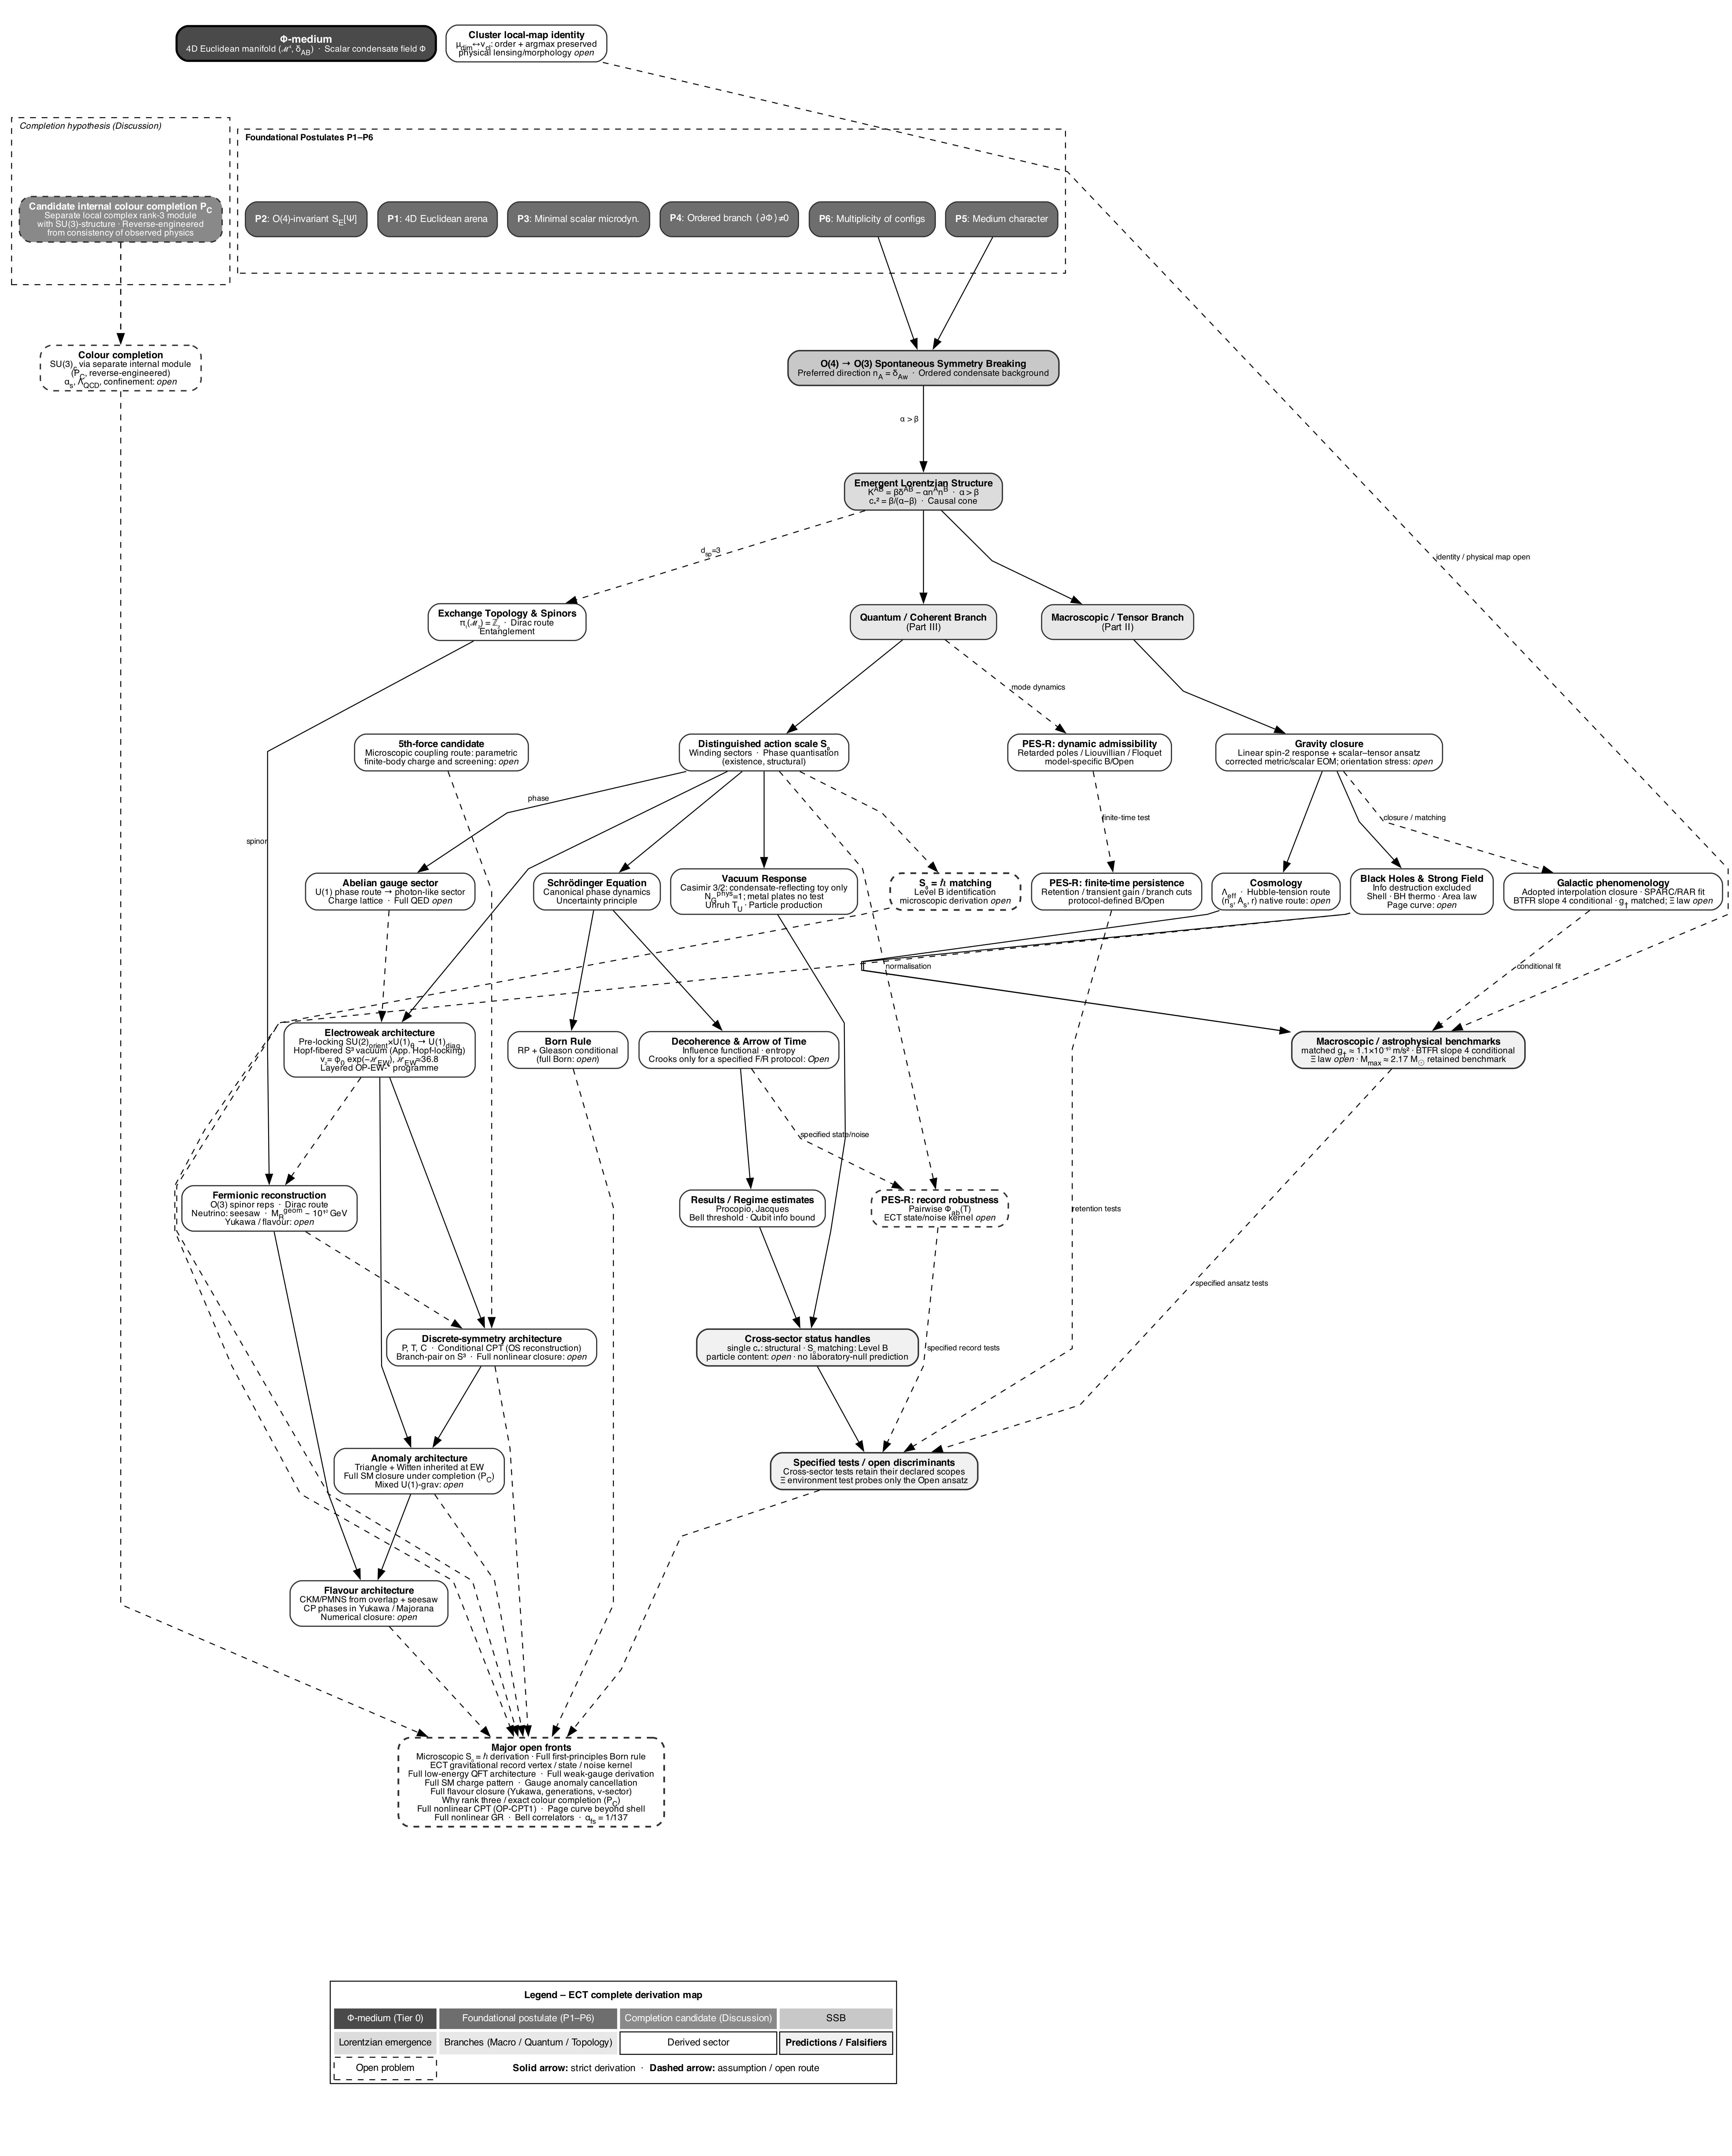
\includegraphics[width=\textwidth]{fig_ect_derivation_map_pop.png}
\caption{Complete ECT derivation map. The full logical architecture from the $\Phi$-medium and the six postulates through all four Parts of the theory. Colours indicate postulates (dark), phenomenological inputs (grey), Level~A (light grey), Level~B (white), and Open (dashed).}
\label{fig:pop_fullmap}
\end{figure}

Figure~\ref{fig:pop_fullmap} shows the complete derivation architecture of ECT.


\section{Проблемы физики, адресуемые ECT}

Within its framework, ECT addresses several well-known open problems of modern physics:

\begin{enumerate}
\item \textbf{Unification of quantum mechanics and gravity.} Both emerge from the same ordered condensate. The unification is architectural, not forced (\emph{A/B}).

\item \textbf{The origin of time.} Why does spacetime have signature $(-,+,+,+)$? Derived from $O(4)\to O(3)$ SSB (\emph{A}).

\item \textbf{The dark matter problem.} No DM particle has been detected despite decades of searches.  The specified galactic interpolation does not require a particle halo in its fitted channel (\emph{C}), but its source/force map is not derived and hidden-sector particles are not excluded.

\item \textbf{The cosmological constant problem.} The leading ordered sector blocks the direct vacuum-baseline channel (Level~A); the loop channel is $H_\Lambda$-conditional and the observed $\rho_\Lambda$ remains a Level-C infrared matching problem.

\item \textbf{The Hubble tension.} $>5\sigma$ discrepancy. ECT provides structural alleviation through evolving $G_{\rm eff}$ (\emph{sign: A; magnitude: B}).

\item \textbf{JWST early galaxies.} A scalar-only diagnostic closure with larger fitted $G_{\rm eff}$ and an additional effective term can accelerate structure formation (\emph{C}); no orientation contribution is computed.

\item \textbf{Baryon asymmetry.} Sakharov-compatible ingredients are closure-level (B); $\eta_B\sim9\times10^{-10}$ is an external benchmark and the ECT-native derivation is Open.

\item \textbf{Black-hole information paradox.} Fundamental information destruction is absent at the postulate level; a finite-memory shell toy gives Page-curve-like behaviour (\emph{B}), while a constructive ECT Page curve remains Open.

\item \textbf{The measurement problem.} Decoherence supplies a Level~B suppression route; pointer-basis selection, single outcome, and the update theorem remain Open.

\item \textbf{The origin of quantum mechanics.} The condensate supplies structural/conditional reconstruction routes; Born weights require C1--C3 and the exact theorem remains Open (\emph{A/B/Open}).

\item \textbf{The arrow of time.} Retarded backbone is structural; monotonic entropy growth requires the Level~B environmental closure.

\item \textbf{The need for inflation.} Four non-inflationary structural/conditional routes are identified; branch selection and the quantitative spectrum remain Open (\emph{A/B/Open}).

\item \textbf{The hierarchy problem.} $M_{\rm Pl}/M_{\rm EW} \sim 10^{16}$ addressed through running coupling (\emph{B/Open}).
\end{enumerate}

The breadth of problems addressed from a single starting point is a distinctive feature of the framework.


\section{Заключение}

ECT is an attempt to place spacetime, gravity, and quantum behaviour within a single pre-spacetime framework. In its current form, some parts of this programme are structural results, some are closure-dependent effective constructions, and some remain open.

\textbf{What is established structurally (Level~A):}
Lorentzian signature from $O(4) \to O(3)$ SSB, the ordered-branch causal-cone structure, the equation hierarchy, and the retarded backbone of the arrow of time are the strongest structural entries. The empirical identification $c_*=c$ is matching; BTFR slope~4 is B/C algebra inside G; the horizon/flatness/monopole routes are mixed A/B/Open; black-hole information destruction is absent only at the postulate level.

\textbf{What is obtained at effective/closure level:}
At Level~B lie declared matching/closure results; orientation stress remains Open.  At Level~C, the SPARC sample medians are $\chi_r^2\approx2.7$ (fixed $M/L$) and $\approx1.4$ (free $M/L$), versus the quoted MOND comparator $\approx3.1$ on comparable footing.  The scalar-to-G map, any $\Xi$ law, exact Born theorem, black-hole coefficient/Page curve, and complete dark-sector closure remain Open.

\textbf{What remains an open programme:}
Three fermion generations; Yukawa hierarchy; $\alpha = 1/137$; renormalisability; Born rule as first-principles theorem; Bell correlators; complete BH evaporation; gradient condensation from bare P3.

The minimal galactic fit contains no particle-halo term, and the present architecture does not take a rigid cosmological constant, an inflaton, separate quantum axioms, or an ad hoc collapse mechanism as independent starting inputs.  This does not exclude hidden-sector particles, and several replacement routes remain closure-level or Open.

Whether ECT ultimately becomes a viable theory of nature or remains a productive conceptual laboratory, it does something valuable: it formulates a testable programme in which spacetime, gravity, and quantum mechanics may share a common substrate while their derivation statuses remain explicit, and it identifies the specific structures --- gradient condensation, compact-phase topology, orientation stiffness, and the Principle of Euclidean Stationarity --- that make this possible.

If even partly correct, the deepest truth about reality is not that the universe \emph{contains} time, but that under the right conditions, the universe \emph{creates} it.

\vspace{2em}
\noindent\rule{\textwidth}{0.5pt}

\noindent\textbf{Note.}
This article is a narrative companion to:
\emph{``Euclidean Condensate Theory (ECT): Emergence of Spacetime,
Quantum Mechanics, and Gravity from Spontaneous $O(4)$ Symmetry
Breaking''} by Valeriy Blagovidov (2026).
Full preprint: \href{https://doi.org/10.5281/zenodo.18917930}{doi:10.5281/zenodo.18917930}.

\medskip
\centerline{\url{https://github.com/chufelo/ECT-preprint-code}}
\medskip
\centerline{Zenodo: \url{https://doi.org/10.5281/zenodo.18917930}}

\end{document}
